\documentclass[10pt]{article}
\usepackage[margin=1in]{geometry}
\usepackage{graphicx}
\usepackage{booktabs}
\usepackage{multirow}
\usepackage{amsmath}
\usepackage{amssymb}
\usepackage{xcolor}
\usepackage{hyperref}
\usepackage{caption}
\usepackage{subcaption}
\usepackage{enumitem}
\usepackage{microtype}
\hypersetup{colorlinks=true,linkcolor=black,citecolor=blue,urlcolor=blue}

\graphicspath{{figures/}}

\title{Beta-Testing Monopoly: \\Closed-Loop Game-Design Optimisation
       over a Diverse Strategy Pool}
\author{Selim Emir Can (selimcan@stanford.edu) \and Alaz Cig (alaz@stanford.edu)}
\date{2026-06-06}

\begin{document}
\maketitle

\begin{abstract}
We present a closed-loop, agent-driven beta-testing workflow for game
design, instantiated on Monopoly. A genetic algorithm searches a 66-dim
board design space (per-property cost and rent multipliers and a 22-bit
keep-mask) under a composite objective combining fairness, game length,
draw rate, and inter-player money transfer, evaluated against a fixed
pool of 30 parametric rule-based strategies. A second agent class, a
1.5B-parameter instruction-tuned LLM (Qwen2.5-1.5B) wrapped in a
structured echo-validated prompt, re-evaluates the same boards as an
independent cross-class probe. The rule-based GA improves the composite
score by approximately 40\% over the default board for both 2 and 3
players. Single-objective ablations confirm that every term in the
composite is non-redundant. A $2p\!\leftrightarrow\!3p$ cross-evaluation
at $n{=}1000$ exposes a fairness gap that does not vanish with budget.
The LLM probe reproduces the rule-based directional ranking with zero
model-side hallucinations across 2{,}288 calls under structured
validation. Re-running the GA with the LLM in the evaluator role yields
a board that beats the default but loses to the rule-based winner under
the diverse pool: the fairness gap is $0.20$ vs.\ $0.379$ at 2p and
$0.05$ vs.\ $0.404$ at 3p, diagnosing the blind spots of any
single-personality evaluator. Code, logs, and figures:
\url{https://github.com/Selim-Emir-Can/CS348K-proj}.
\end{abstract}

% =====================================================================
\section{Background and setup}\label{sec:bg}
% =====================================================================

\paragraph{The problem.} Game designers face combinatorial design
spaces that human playtesting cannot cover. Tabletop Monopoly is a
sharp testbed for the agent-assisted alternative: a small but rich
parameter space and well-known balance issues (games drag on,
single-property luck dominates, two-player play is unbalanced). The
goal of this project is not to ``solve'' Monopoly but to demonstrate a
reproducible designer-facing beta-testing loop:
\begin{quote}
\textbf{Parameterise environment} $\to$ \textbf{evaluate against a
diverse agent population} $\to$ \textbf{compare agreement across
agent classes} $\to$ \textbf{shortlist candidate designs} $\to$
\textbf{send only the most informative cases to human playtest.}
\end{quote}

\paragraph{Inputs and outputs.} The pipeline takes a board configuration
$\theta \in \mathbb{R}^{44} \times \{0,1\}^{22}$ (22 cost multipliers,
22 rent multipliers, 22 keep-mask bits) and produces (i) a scalar
composite score plus a per-component metric tuple
$(\overline{F}, F_{\max}, \overline{R}, \overline{D}, \overline{T})$
estimated over $100$ games against the strategy pool, and (ii) a
decision-quality artefact (per-strategy heatmap, per-game JSONL, or
per-decision LLM log) that lets the designer audit \emph{why} $\theta$
scored as it did.

\paragraph{Goals and constraints.} The optimiser minimises a weighted
sum of five design qualities (Eq.~\ref{eq:score}), chosen so that no
single term dominates: mean pair-fairness $\overline{F}$, worst-pair
fairness $F_{\max}$, length deviation $|\overline{R}-R^{*}|/R^{*}$,
mean draw rate $\overline{D}$, and player-to-player money-transfer
deviation $|\overline{T}-T^{*}|/T^{*}$. Hard constraints: every
candidate runs end-to-end at the per-property cost/rent bounds
$[0.5, 2.0]$, retains both utilities and railroads, and finishes or
truncates within $200$ rounds. Soft constraints: total wall-clock
budget under $30$ minutes on a single CPU ($\approx 6$ ms/game) for the
rule-based pipeline, and under $6$ hours on a single $12$ GB GPU for
the LLM probe.

\begin{equation}\label{eq:score}
\text{score}(\theta) \;=\;
   w_{\text{fair}} \overline{F} \;+\;
   w_{\text{fmax}} F_{\max} \;+\;
   w_{\text{len}}  \tfrac{|\overline{R}-R^{*}|}{R^{*}} \;+\;
   w_{\text{draw}}\overline{D} \;+\;
   w_{\text{money}}\tfrac{|\overline{T}-T^{*}|}{T^{*}}
\end{equation}
Defaults: $w=(1,\,0.5,\,0.5,\,0.3,\,0.3)$, $R^{*}=60$ rounds,
$T^{*}=100$ \$/round.

\paragraph{Hypothesis.} The falsifiable claim of the project is that a
candidate board's directional ranking under a 30-strategy parametric
pool matches its directional ranking under an independent agent class
(a 1.5B-parameter LLM with a deterministic per-field state validator),
at a per-decision hallucination rate below $1\%$. This sits between
``a single trained agent ranks designs'' (insufficient for fairness)
and ``agents predict human win-rates'' (likely hopeless, and not what a
designer needs); it is precisely the claim required to use agent
feedback as a beta-testing surrogate.

\paragraph{The crux.} The hard part of the project is neither the GA
over a 66-dim board space nor the LLM plumbing; it is the question of
\emph{what evaluates a candidate board} in the absence of human
playtesters. A single trained agent (RL or LLM) used as an oracle
collapses ``design quality'' to one playstyle's quirks: a board that
scores well against an aggressive builder may be obviously broken
against a cash hoarder. The honest alternative is to evaluate against a
\emph{population} of strategies, but the strategy space we care about
is continuous (17 knobs: 5 continuous, 4 boolean, an 8-bit
colour-group mask), so the real question is \emph{which strategies,
and how many}. The project's load-bearing design choice is the
discretisation: 10 hand-designed archetypes (\textsl{AggressiveBuilder,
CashHoarder, Trader, RailroadKing, LowCostOnly, HighCostOnly, Balanced,
Passive, Bully, RiskAverse}) chosen to span qualitatively different
playstyles, plus 20 samples drawn once from the parametric space with
a fixed seed to fill the gaps between them. Thirty strategies is small
enough that 100 games per candidate over 200 candidates fits in
$\sim 25$ minutes on a single CPU, and large enough that worst-case
fairness across the pool is a meaningful objective rather than a coin
flip on one matchup. A secondary technical challenge, addressed as part
of the cross-class validation rather than the central contribution, is
making a small instruction-tuned LLM usable as an independent agent
class without hallucinations leaking into the metrics; the solution is
a structured \texttt{STATE/ECHO/REASON/ANSWER} prompt with
deterministic per-field state validation and a bounded retry budget,
reported with its failure modes (Section~\ref{sec:llm}).

% =====================================================================
\section{Approach}\label{sec:approach}
% =====================================================================

We started from a single-process Monopoly core game loop with a
\texttt{Player} base class, a YAML round-trip \texttt{GameConfig}, and
a small set of rule-based player subclasses, plus pretrained
Qwen2.5-1.5B-Instruct~\cite{qwen25} weights from Hugging Face. Every
piece of the optimisation loop, the strategy pool, the design-space
encoder, the per-game stat collection, and the LLM integration was new
work for this project.

The optimisation stack lives under \texttt{monopoly/optimizer/} and
\texttt{monopoly/scripts/}. \texttt{ParametricPlayer} together with
\texttt{ParametricPlayerSettings} subsumes every existing rule-based
subclass under a single 17-knob agent (5 continuous, 4 boolean, 8-bit
colour-group mask). \texttt{strategy\_pool.py} produces the 30-strategy
pool described in Section~\ref{sec:bg}, deterministic via a fixed seed
and saved once for reuse across runs. \texttt{design\_space.py} maps a
66-dim vector to a fresh \texttt{GameConfig} by applying per-property
multipliers to \texttt{cost\_base}, \texttt{cost\_house},
\texttt{rent\_base}, and \texttt{rent\_house}, and physically removing
properties whose keep-bit is zero (structurally shortening the lap
rather than substituting \texttt{FreeParking}); the identity vector is
the default board. \texttt{simulate.py} is a thin re-implementation of
the inner game loop that returns a per-game stat dict (winner, rounds,
bankruptcy map, inter-player transfer total) instead of only logging;
inter-player cash flow is captured via a context-manager monkey-patch
of \texttt{Player.pay\_money}, with non-player payments (taxes, fines,
salary) excluded, and trade calls are capped at 5 per (player, turn)
to break an unbounded loop in upstream code. \texttt{search.py}
implements both random search and a GA (population 20, 10 generations,
tournament selection $k{=}3$, uniform crossover, $\sigma{=}0.1$
Gaussian mutation on continuous dims, 1-bit-flip mutation on the
keep-mask, elitism 2); both produce identical JSONL.

The LLM layer is a single subclass \texttt{LLMPlayer} in
\texttt{agents.py}: a pre-filter avoids LLM calls when affordability
or cash floor decides the action, the prompt has the
\texttt{STATE/ECHO/REASON/ANSWER} structure described in
Section~\ref{sec:bg}, and the validator parses the model's
\texttt{ECHO} block with a multiline regex and equality-checks each of
the 10 fields against ground-truth state (with a $\$0.50$ tolerance to
absorb float drift). On any echo mismatch the player retries, up to
\texttt{MAX\_RETRIES=4}, replaying prior assistant turns plus a
corrective message naming the mismatched fields. Every decision is
logged via the \texttt{decision\_log\_path} kwarg; the log records the
prompt, raw response, parse path, ms elapsed, generation metadata,
echo mismatches, and the full attempt list.

Three design decisions did most of the work for the evaluation
sections that follow. The validator-and-retry stack is treated as
\emph{part of the probe} rather than infrastructure around it, and we
report both v1 and v2 versions because an LLM with a broken validator
is a measurably different design probe than one with a working
validator (Section~\ref{sec:llm}). Shared random numbers across
candidates make GA convergence visible at $100$ games per candidate
rather than the $\sim 1000$ that uncorrelated evaluations would
require: every candidate is scored on the same $10$ matchups
$\times$ $10$ seeds, and an unchanged design vector yields
byte-identical metrics. Finally, the agent population is the
evaluator, not the oracle: a single agent collapses design quality to
its own quirks, while the 30-strategy pool exposes worst-case
fairness as a first-class objective.

The end-to-end pipeline is driven by four scripts.
\texttt{scripts/optimize\_board.py} runs the rule-based search and
emits one JSONL line per evaluation. \texttt{scripts/cross\_eval.py}
runs designs through both player-count harnesses at $n{=}1000$.
\texttt{scripts/strategy\_heatmap.py} produces $30{\times}30$
strategy-vs-strategy win-rate matrices on any chosen design.
\texttt{scripts/eval\_llm\_on\_boards.py} runs the all-LLM-seat probe
with per-decision logging, and \texttt{scripts/optimize\_board\_llm.py}
re-runs the GA with the LLM in the evaluator role.

% =====================================================================
\section{Evaluation and results}\label{sec:eval}
% =====================================================================

\paragraph{Definition of success.} The project is successful if all
three of the following hold:
\begin{enumerate}[leftmargin=1.4em,itemsep=1pt]
\item the GA finds a board that improves the composite score over the
default by a margin larger than the noise floor, verified at the
optimum with $n{=}1000$ and $95\%$ Wilson intervals on every metric;
\item single-objective ablations show that each of the five composite
terms drives a different optimum, establishing that the objective is
non-redundant;
\item an independent agent class (LLM under structured ECHO
validation) reproduces the same directional ranking on the optimised
boards, at a per-decision hallucination rate below $1\%$.
\end{enumerate}
A weaker fourth claim, treated as diagnostic rather than headline, is
that running the GA with the LLM as evaluator should produce a board
that behaves \emph{plausibly} under the rule-based pool, even if it
loses to the rule-based winner.

\paragraph{Experimental setup.} The strategy pool is 30 parametric
players (10 archetypes plus 20 sampled), pickled once with a fixed
seed. For each player count $n\in\{2,3\}$ we draw 10 evaluation
matchups under diversity constraints: every archetype appears in at
least one matchup, and at least 3 matchups include a sampled
strategy. Each candidate is scored on $10\times 10 = 100$ games with
seeds shared across all candidates, so an unchanged design vector
yields byte-identical metrics. Hardware: a single CPU at
$\approx 6$ ms/game for the rule-based stack; a single $11$ GB GPU
locally for LLM games at
$\approx 6$--$10$ s/decision. Total games for the entire study:
$\approx 165$k for the rule-based pipeline, $\approx 2300$ for the
LLM cross-class probe, and $\approx 2000$ for the LLM-driven GA and
its cross-evaluation.

\subsection{Default-board baseline and search}\label{sec:baseline}

The default board is the identity vector under the encoder. It scores
$\sim 0.61$ on the composite at 2p and $\sim 0.71$ at 3p (full
metrics in \texttt{logs/optimizer/default\_baseline.json}); these are
the reference points every optimisation result is compared against,
with $95\%$ Wilson intervals computed over the 100-game evaluation.

\begin{figure}[h!]
\centering
\begin{subfigure}[t]{0.48\linewidth}\centering
  
\includegraphics[width=\linewidth]{convergence_2p.png}
  \caption{2 players}
\end{subfigure}\hfill
\begin{subfigure}[t]{0.48\linewidth}\centering
  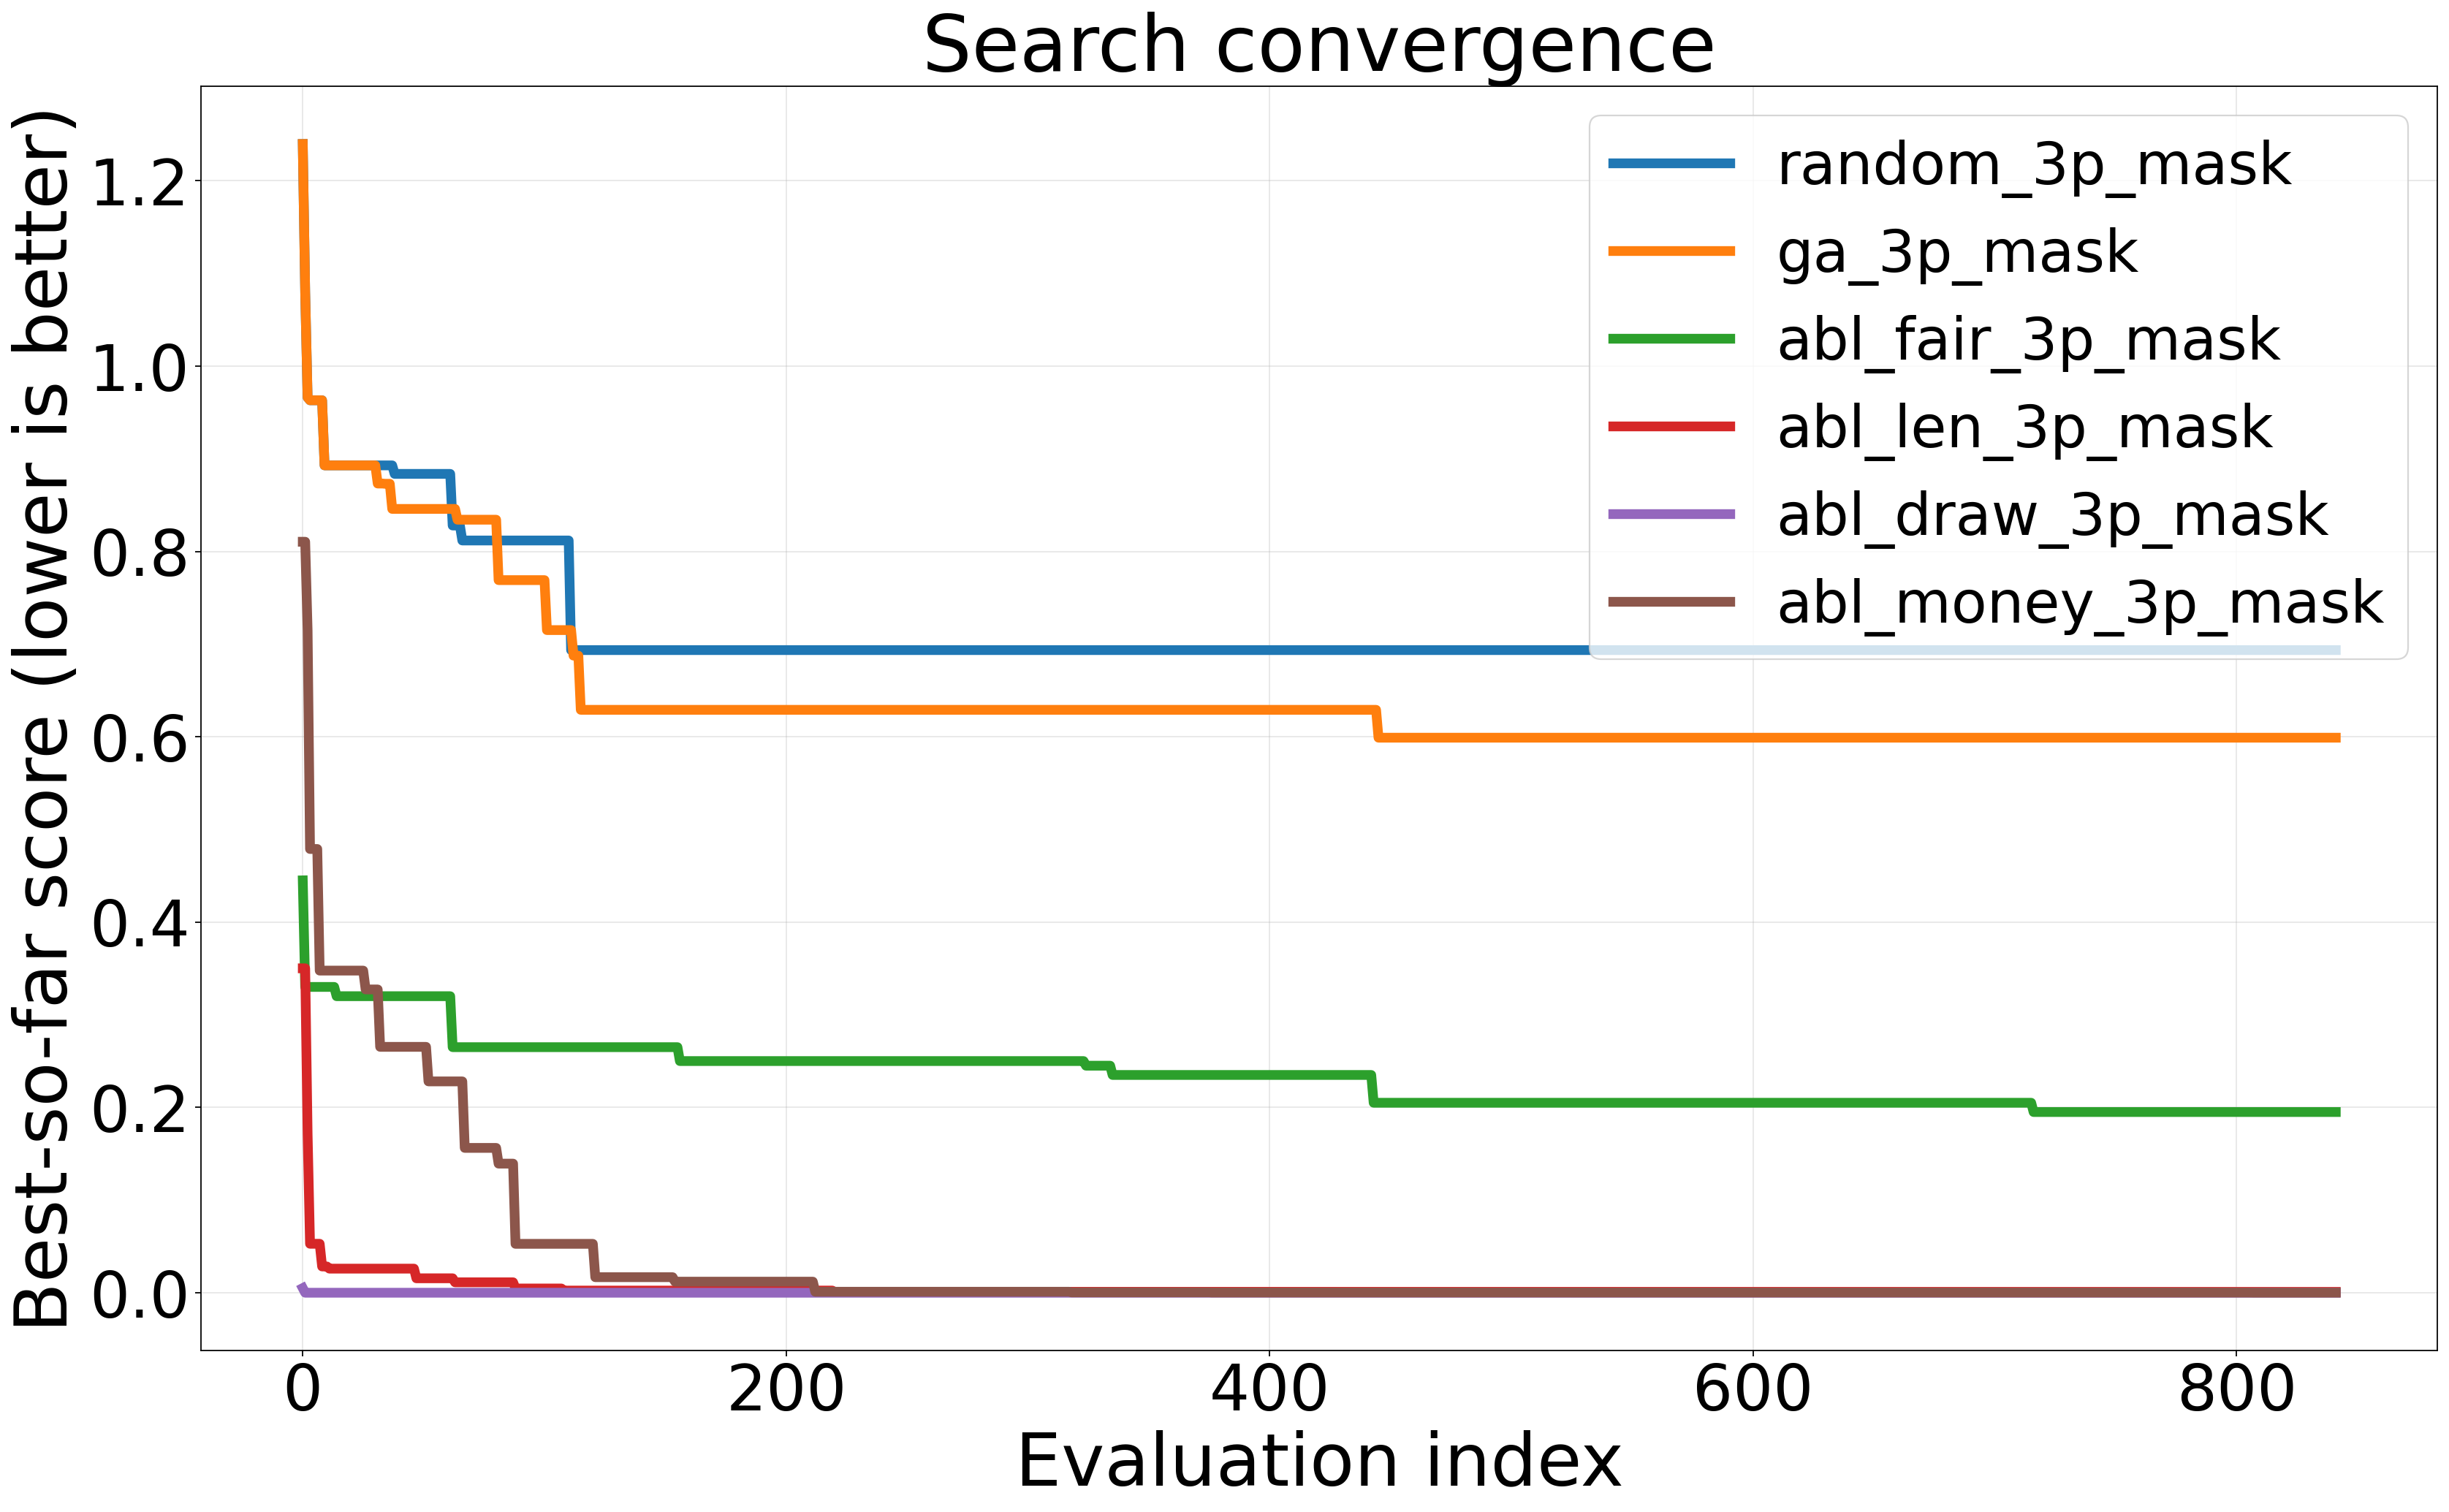
\includegraphics[width=\linewidth]{convergence_3p.png}
  \caption{3 players}
\end{subfigure}
\caption{\textbf{Optimisation works, but problem framing drives most
of the lift.} Best-so-far composite score (lower is better) over the
candidate-evaluation budget for the GA and random search, at 2 and 3
players. The horizontal dashed line is the default board's score
under the same evaluator. The GA finishes $\approx 16\%$ ahead of
random search at both player counts, but the gap between either
curve and the default line is several times larger: the headline
improvement comes from the choice of objective and evaluator, not
from the choice of search algorithm.}
\label{fig:conv}
\end{figure}

The GA outperforms random search consistently across the run, but not
by an order of magnitude (Figure~\ref{fig:conv}). The larger lift
comes from problem framing rather than optimiser cleverness: the
composite objective, the fixed strategy pool, and shared random
numbers across candidates make random search on this problem already
a strong baseline. This is consistent with a more general observation
about system-design problems, where the bottleneck is usually problem
formulation rather than search.

\subsection{Single-objective ablations}\label{sec:ablation}

We ran five ablations per player count, each setting one weight to
$1$ and the others to $0$ (\textit{fairness-only, length-only,
draw-only, money-only, combined}), and reported best-so-far
convergence and the full metric tuple at the optimum. Each ablation
reaches a different optimum: the length-only run drives $\overline{R}$
to within $\approx 1$ round of $R^{*}=60$ but degrades fairness, while
the fairness-only run nearly halves $\overline{F}$ but inflates draws.
The per-aspect heatmaps in Figure~\ref{fig:multipliers} show the
ablations carving visibly different shapes in the cost-multiplier,
rent-multiplier, and keep-mask sub-spaces. The composite is therefore
non-redundant: if any two terms drove the optimiser toward the same
board, the corresponding ablations would have near-identical metrics,
which they do not.

\begin{figure}[h!]
\centering
\begin{subfigure}[t]{0.31\linewidth}\centering
  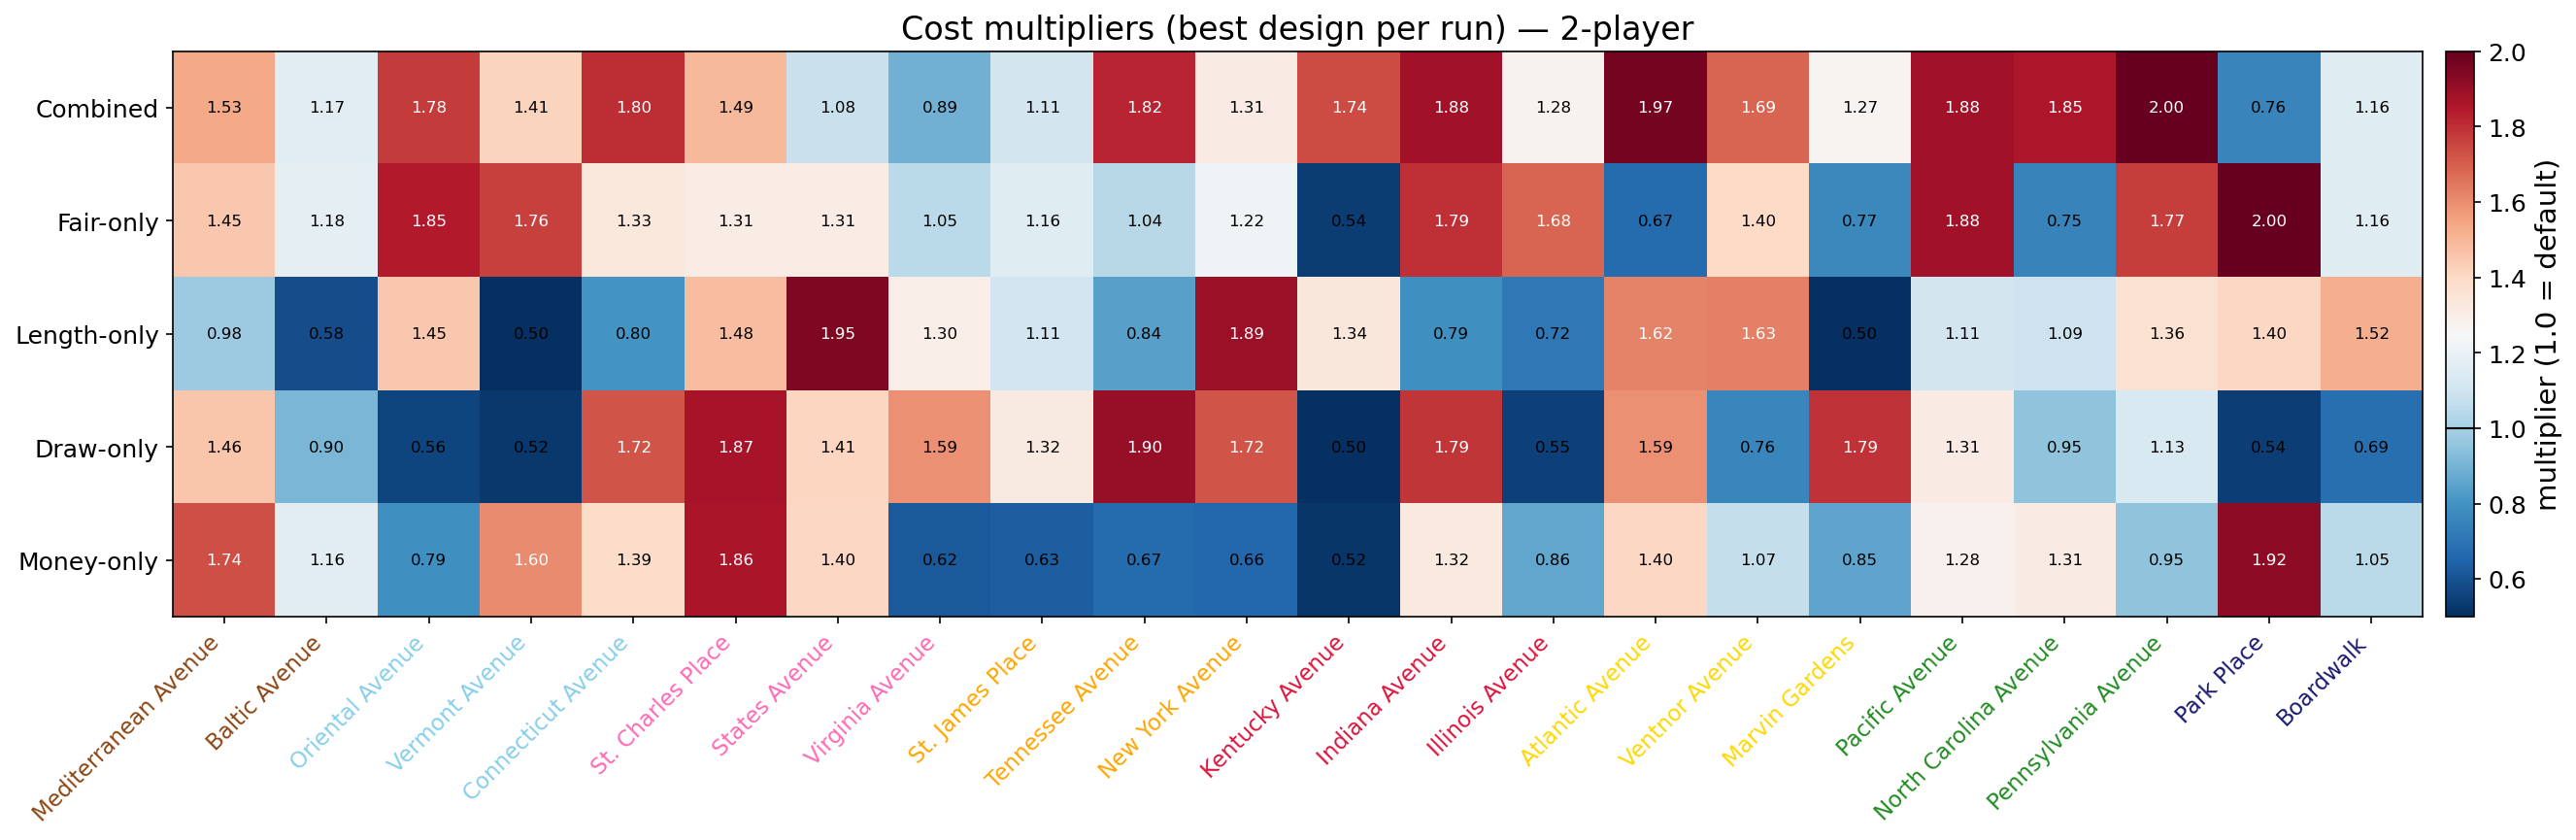
\includegraphics[width=\linewidth]{cost_multipliers_2p.png}
  \caption{cost mult.\ (2p)}
\end{subfigure}\hfill
\begin{subfigure}[t]{0.31\linewidth}\centering
  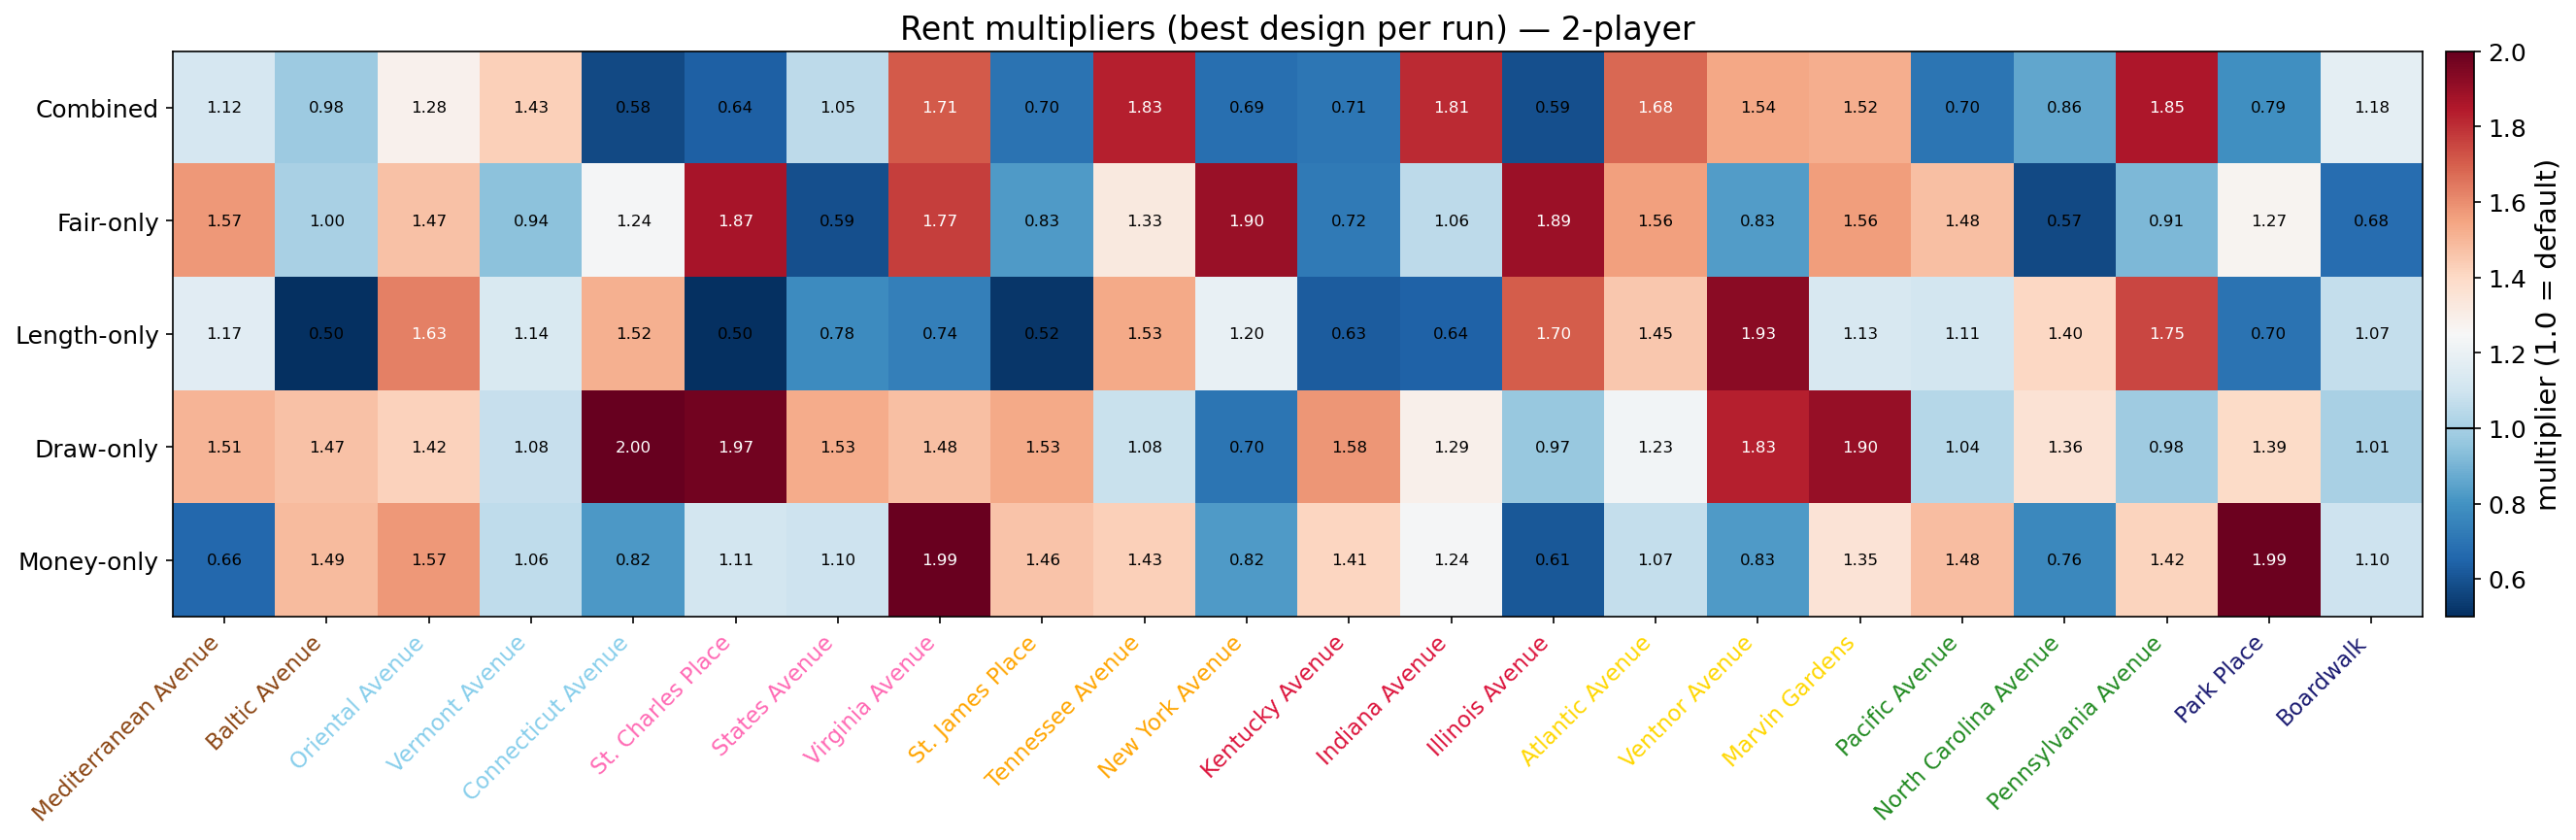
\includegraphics[width=\linewidth]{rent_multipliers_2p.png}
  \caption{rent mult.\ (2p)}
\end{subfigure}\hfill
\begin{subfigure}[t]{0.31\linewidth}\centering
  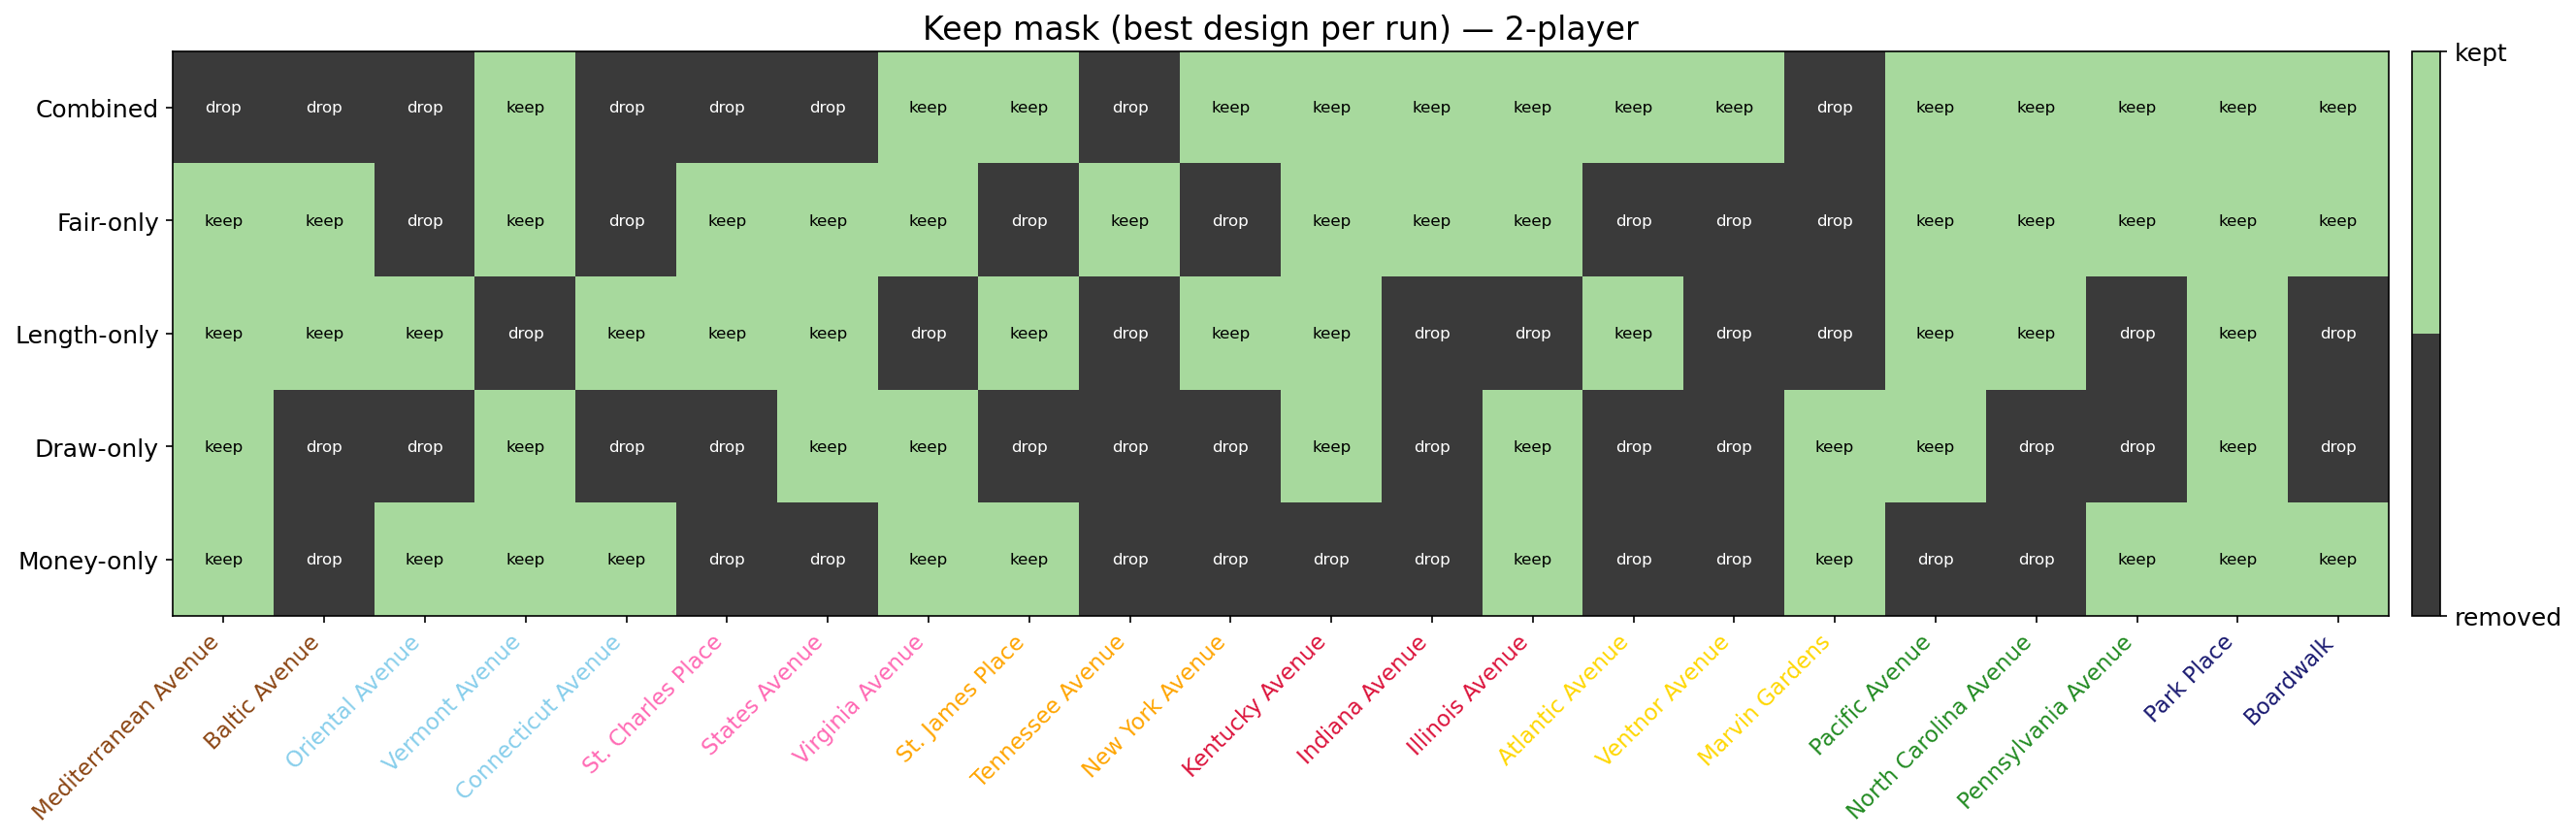
\includegraphics[width=\linewidth]{keep_mask_2p.png}
  \caption{keep-mask (2p)}
\end{subfigure}
\caption{\textbf{Each ablation carves a different shape in design
space (2p).} Per-property cost multiplier (a), rent multiplier (b),
and keep-mask bit (c) at the optimum of each GA run. Within each
panel, rows are the 22 ownable properties in board order and columns
are the five ablations (\textit{fairness-only, length-only,
draw-only, money-only, combined}). If any two ablations drove the
optimiser to the same board, those columns would be near-identical;
the visible inter-column variation is the empirical evidence that
the composite objective is non-redundant.}
\label{fig:multipliers}
\end{figure}

\subsection{$2p\!\leftrightarrow\!3p$ cross-evaluation}\label{sec:cross}

We took the combined-objective winner from each player-count regime
and re-evaluated it under the other harness at $n{=}1000$
(Table~\ref{tab:cross}, Figure~\ref{fig:pareto}). Two findings carry
weight beyond the headline improvement over the default.

\begin{table}[h!]
\centering
\small
\begin{tabular}{llrrrrrr}
\toprule
Design & Eval & score\,$\downarrow$ & $\overline{F}$\,$\downarrow$ & $F_{\max}$\,$\downarrow$ & rounds\,$(\!\to\!60)$ & draw \%\,$\downarrow$ & transfer\,$(\!\to\!100)$ \\
\midrule
default board    & 2p & 1.463 & 0.454 & 0.940 & 103.9 &  7.4 &  49.7 \\
default board    & 3p & 1.230 & 0.412 & 0.680 & 110.8 & 17.6 &  99.4 \\
\addlinespace
GA-2p winner     & 2p & \textbf{0.998} & 0.323 & 0.960 &  69.4 &  2.3 &  63.4 \\
GA-2p winner     & 3p & 0.690 & 0.248 & 0.610 &  71.2 &  3.0 & 111.7 \\
\addlinespace
GA-3p winner     & 2p & 0.954 & \textbf{0.251} & 0.960 &  71.0 &  2.7 &  58.8 \\
GA-3p winner     & 3p & \textbf{0.670} & 0.255 & 0.550 &  72.4 &  4.3 & 107.7 \\
\bottomrule
\end{tabular}
\caption{\textbf{Cross-player-count evaluation at $n{=}1000$ games
per cell.} Wilson $95\%$ CIs on individual win rates are $\pm 3$pp.
Header arrows: $\downarrow$ means lower is better; $(\!\to\!T)$ means
the target value is $T$ and deviation in either direction is
penalised. Bold cells mark the best (lowest) composite score within
each evaluation regime. The GA-3p winner is the stronger universal
design: its 2p score ($0.954$) is better than the GA-2p winner's
score on its own training regime ($0.998$).}
\label{tab:cross}
\end{table}

The first finding is that the \emph{3p-trained design is the stronger
universal design}. The GA-3p winner under 2p evaluation scores
$0.954$ on the composite, better than the GA-2p winner's score on
its own training regime ($0.998$). The same flip holds on fairness
in isolation ($0.251$ vs.\ $0.323$). This contradicts the intuition
that a design tuned for 2p should be best at 2p, and it has a clean
explanation: a 3p game contains more strategy-vs-strategy
interactions per round, so 3p optimisation implicitly pressure-tests
more matchup patterns. The general principle is that when two
evaluation regimes differ in interaction density, the more demanding
regime tends to produce the more robust design, and optimising under
the harder regime should be the default whenever the cost ratio
allows it.

The second finding is that the \emph{optimisation-set overfit is
small at 2p and effectively zero at 3p}. At the $n{=}100$
optimisation budget the GA-2p winner scored $0.83$ on its training
matchup set; at $n{=}1000$ deployment it scores $0.998$, an overfit
of $\sim 0.17$ (Table~\ref{tab:overfit}). The GA-3p winner shows no
such gap: its training score ($0.67$) and its deployment score
($0.670$) are essentially identical. The contrast traces back to the
same root cause as the first finding: a 3p game contains more
strategy-vs-strategy interactions per round, so each game carries
more signal about a board's design quality, and the same $100$-game
budget is effectively denoised. The headline win over the default
($\sim 0.47$ on the score scale) is several times larger than even
the 2p overfit, so the directional improvement survives re-evaluation
either way; we report both training and deployment numbers rather
than picking the more flattering one.

\begin{table}[h!]
\centering
\small
\begin{tabular}{lccc}
\toprule
Design & training ($n{=}100$)\,$\downarrow$ & deployment ($n{=}1000$)\,$\downarrow$ & overfit\,$\downarrow$ \\
\midrule
GA-2p winner & $0.83$ & $0.998$ & $+0.17$ \\
GA-3p winner & $0.67$ & $0.670$ & $\approx 0$ \\
\bottomrule
\end{tabular}
\caption{\textbf{Optimisation-set vs.\ deployment-set composite
score, on the design's own training regime.} Header arrows:
$\downarrow$ means lower is better. The GA-2p winner has a
$\sim 0.17$ overfit to its $100$-game training matchup set; the
GA-3p winner has none. The training number is read from the GA's
own \texttt{evals.jsonl}, the deployment number from the
corresponding row of Table~\ref{tab:cross}.}
\label{tab:overfit}
\end{table}

The Pareto frontiers in Figure~\ref{fig:pareto} have visibly
distinct shapes (different slope, different knee), so the
cross-evaluation result respects the geometry of the design space
rather than being seed noise.

\begin{figure}[h!]
\centering
\begin{subfigure}[t]{0.48\linewidth}\centering
  
\includegraphics[width=\linewidth]{ga_2p_pareto.png}
  \caption{2p}
\end{subfigure}\hfill
\begin{subfigure}[t]{0.48\linewidth}\centering
  
\includegraphics[width=\linewidth]{ga_3p_pareto.png}
  \caption{3p}
\end{subfigure}
\caption{\textbf{The trade-off surface is real, and its shape depends
on player count.} Each marker is one of the $\sim 200$ candidate
boards evaluated by the GA. The x-axis is mean rounds (target
$R^{*}=60$); the y-axis is mean pair-fairness $\overline{F}$ (lower
is fairer). The combined-objective optimum is the marker on the
lower-left knee of the frontier. The 2p and 3p frontiers have
visibly distinct slopes and knees: a board on one frontier does not
in general lie on the other, which is what makes the
cross-evaluation result (Table~\ref{tab:cross}) a property of the
design space rather than seed noise.}
\label{fig:pareto}
\end{figure}

\subsection{Per-strategy heatmaps: \emph{what} did the optimiser
actually fix?}\label{sec:heatmap}

The composite score averages over only the 10 sampled evaluation
matchups; it can move down even if a different subset of strategy
pairs got worse. The full $30\times 30$ strategy-vs-strategy win-rate
matrix on the optimised board (Figure~\ref{fig:heatmap}, left) and
its difference against the default-board matrix (right) decompose
what the GA actually changed across all $\binom{30}{2}=435$ unique
strategy pairs in the pool.

The headline finding is a separation between \emph{system-level} and
\emph{strategy-level} effects. Mean $|W-0.5|$ across the full
$30\times 30$ matrix is approximately $0.21$ on \emph{both} the
default and the GA-optimised board: per-pair fairness across the
population is essentially unchanged. What the GA \emph{did} change is
the system-level metrics that the composite was minimising. Game
length dropped by approximately $30$ rounds, draw rate fell from
$7.4\%$ to $2.3\%$, and inter-player money transfer rose from $50$
to $63$~\$/round. The optimiser shifted pacing, decisiveness, and
interactivity without altering the skill ordering of the strategy
population.

A related observation is that some matchups are immutable under any
board configuration in the search space. The five most asymmetric
pairs on the GA-2p winner include \textsl{Trader} vs.\
\textsl{RailroadKing} ($100\%$/$0\%$) and \textsl{RailroadKing} vs.\
\textsl{Sampled\_18} ($0\%$/$100\%$). No setting of cost multipliers,
rent multipliers, or keep-mask bits eliminates these; they are
intrinsic to a strategy that refuses to buy $22$ of $28$ ownable
properties, and the GA cannot reach them through the design space.
This is the substantive negative result of the section: board design
is a lever for system-level properties (length, draws,
interactivity), but agent-level dominance is structural to the
strategy pool. Closing those residual gaps requires a strategy-side
intervention (rule changes, matchmaking, or pool curation), not more
search over the design space.

\begin{figure}[h!]
\centering
\begin{subfigure}[t]{0.48\linewidth}\centering
  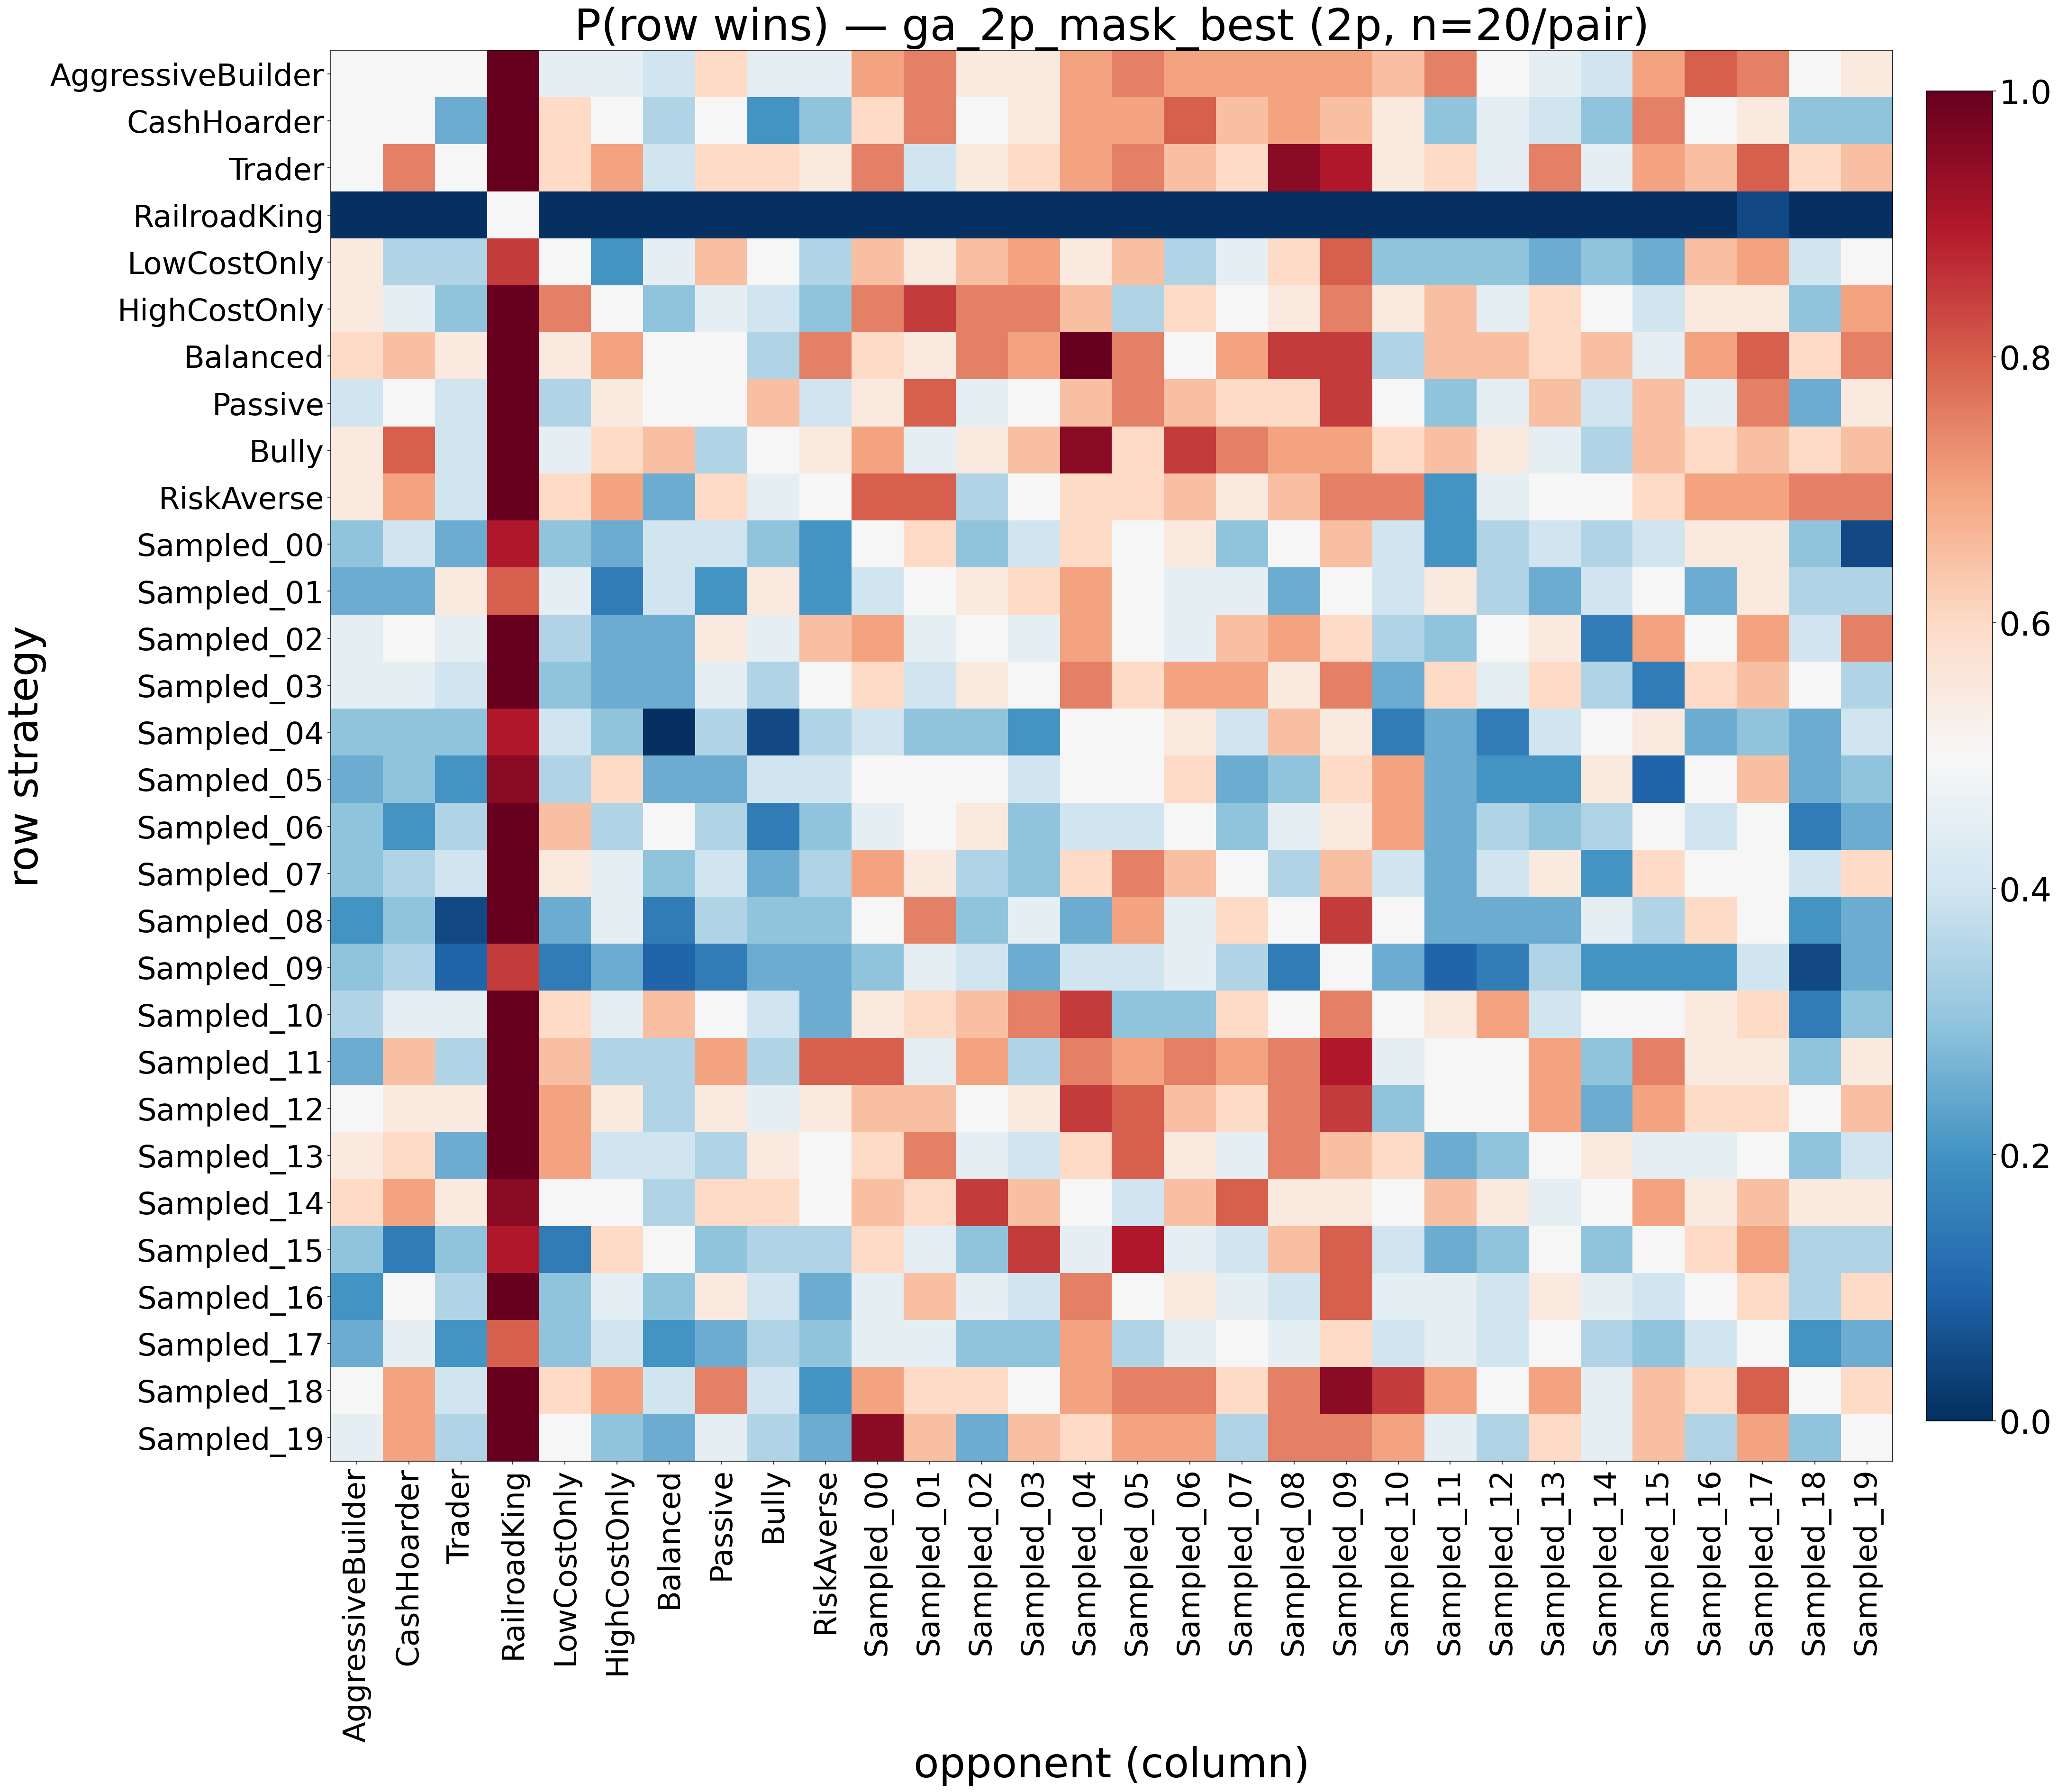
\includegraphics[width=\linewidth]{heatmap_ga2p.png}
  \caption{Optimum (2p)}
\end{subfigure}\hfill
\begin{subfigure}[t]{0.48\linewidth}\centering
  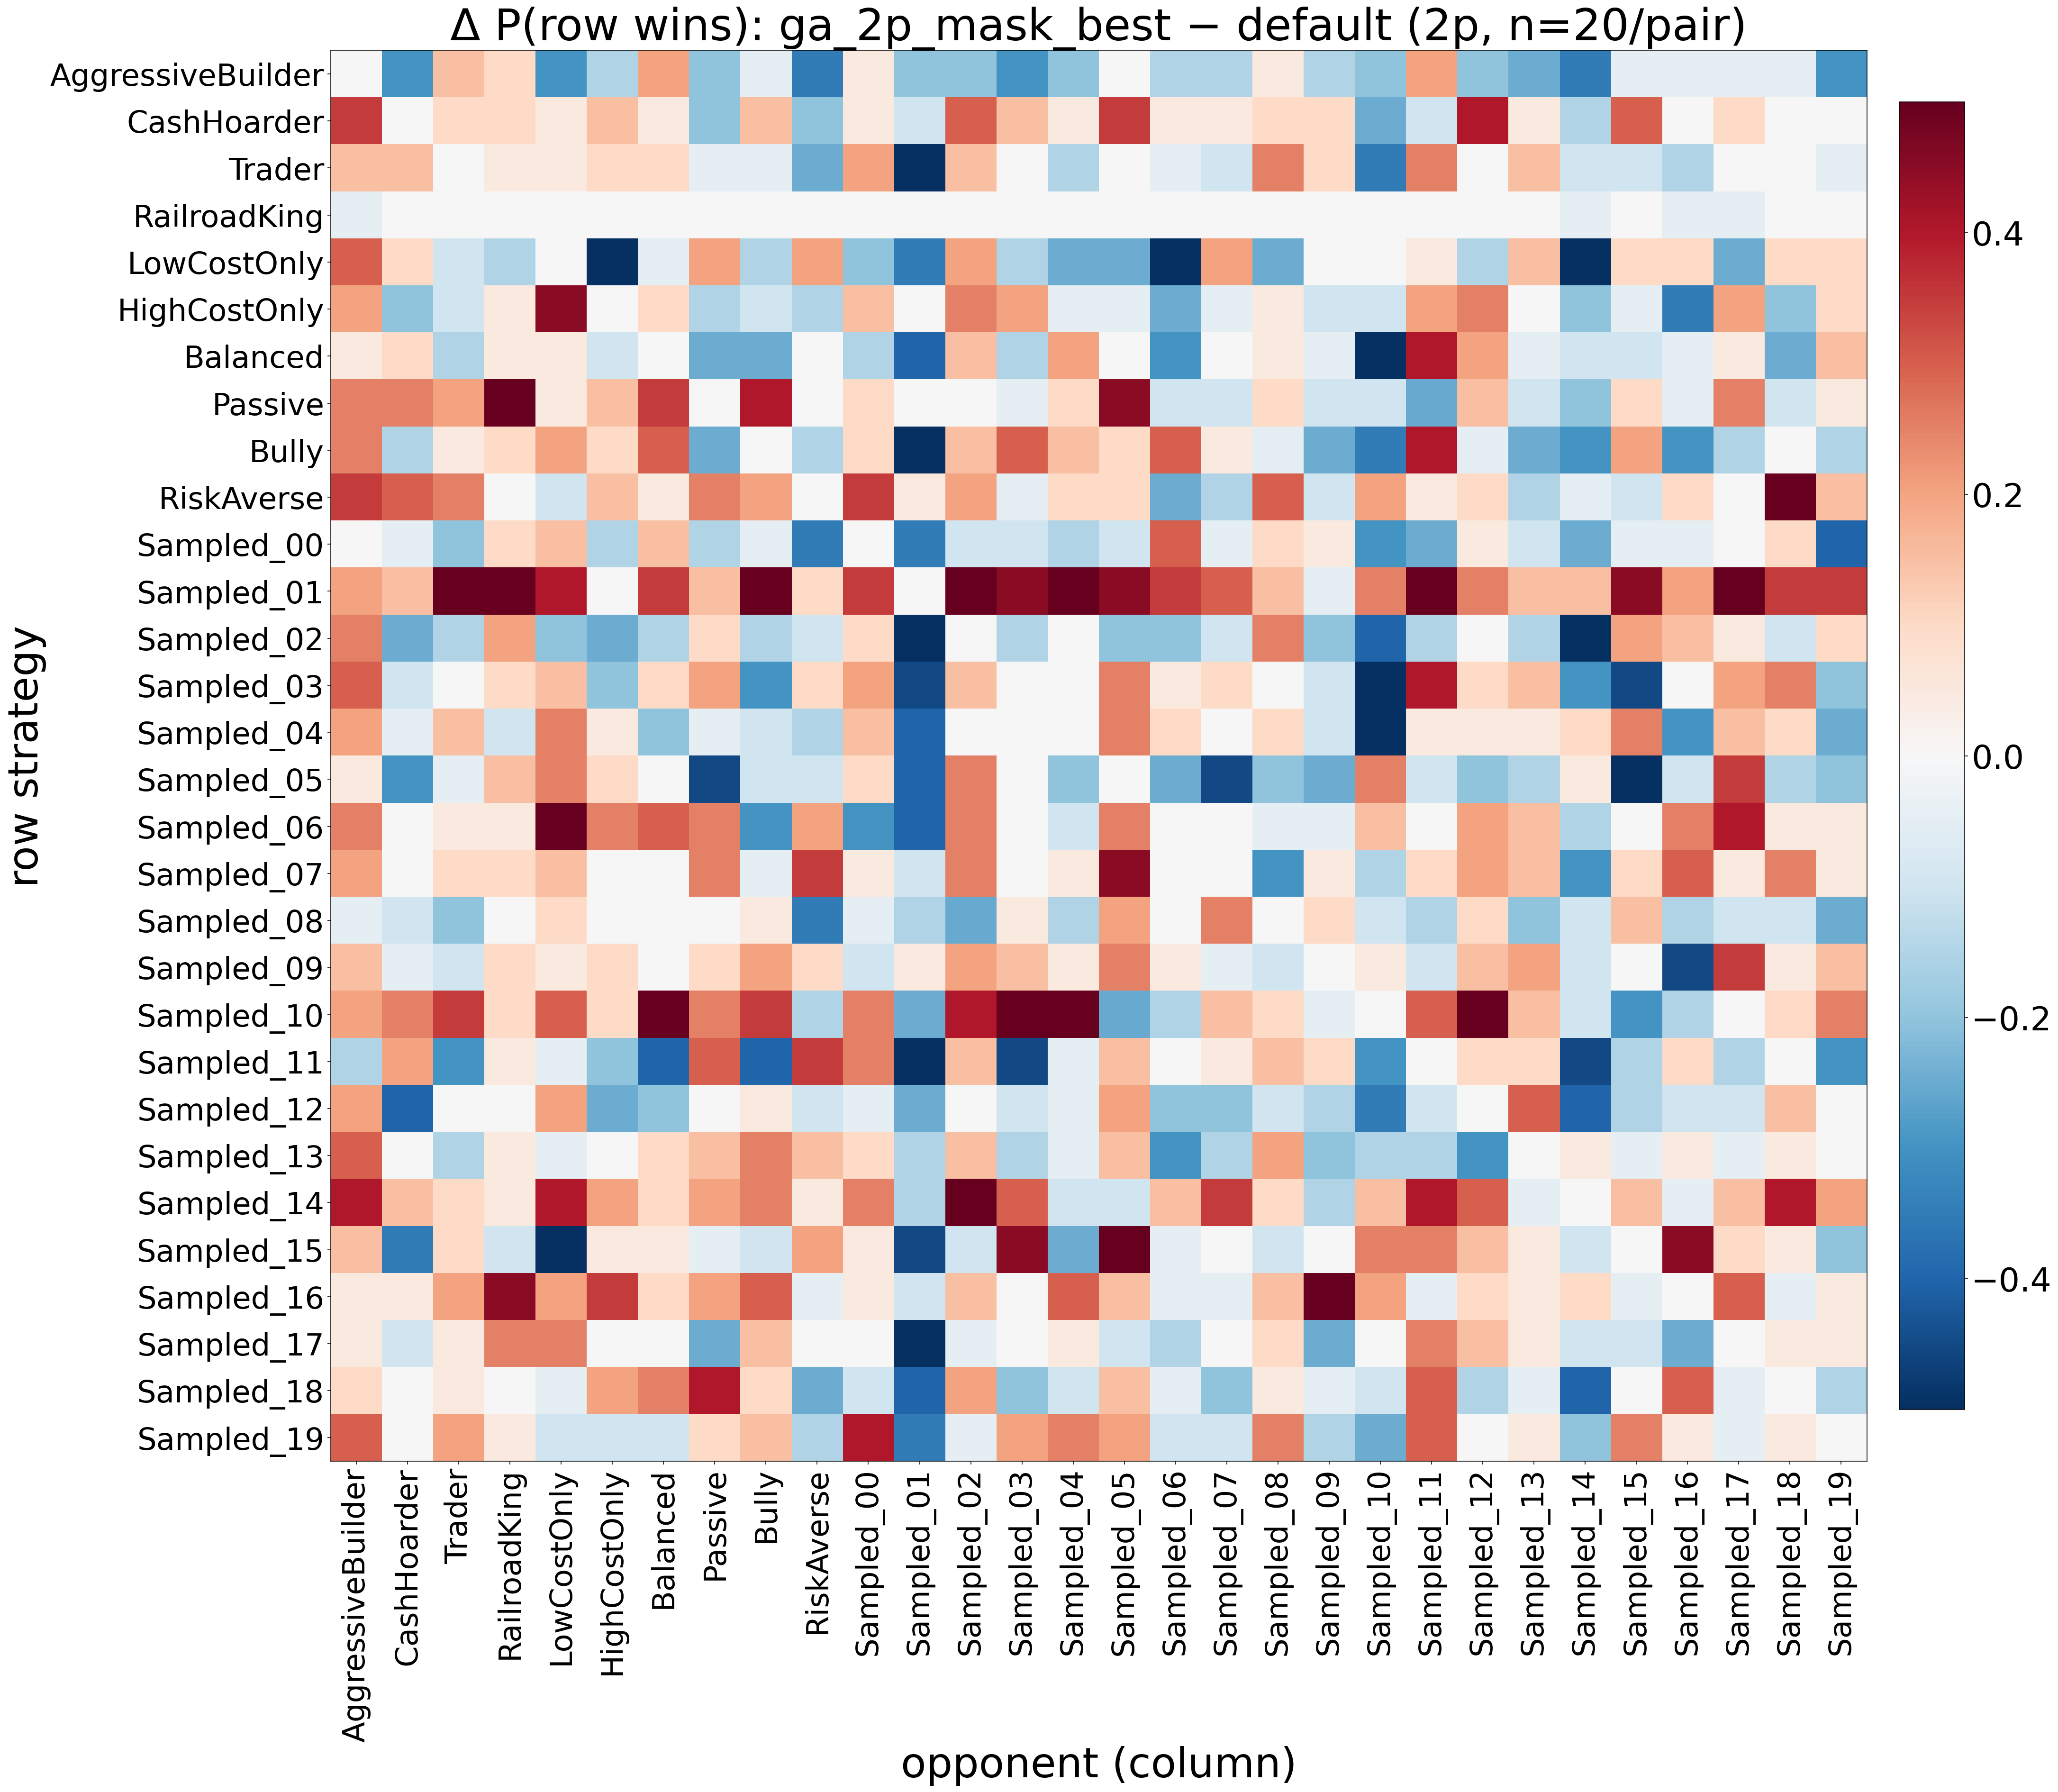
\includegraphics[width=\linewidth]{heatmap_ga2p.diff.png}
  \caption{Optimum minus default (2p)}
\end{subfigure}
\caption{\textbf{$30\times 30$ strategy-vs-strategy win-rate matrices.}
\textbf{(a)}~Win rates on the GA-2p winning board, $P(\text{row beats
column})$; the diagonal is fixed at $0.5$. \textbf{(b)}~Difference
against the default board, centred at zero. Across the full
$\binom{30}{2}=435$ unique pairs, mean $|W-0.5|$ is approximately
$0.21$ on \emph{both} the default and the GA-optimised board:
per-pair fairness is unchanged. The GA improved the system-level
metrics (length, draws, transfer) without altering the
strategy-level skill ordering of the pool.}
\label{fig:heatmap}
\end{figure}

\subsection{LLM cross-class agreement (Phase~C)}\label{sec:llm}

The cross-class probe re-ran 80 games on the optimised boards under
all-LLM seats (Qwen2.5-1.5B-Instruct, greedy decoding) using the
structured \texttt{STATE/ECHO/REASON/ANSWER} prompt. Per-decision logs
record prompt, raw response, parse path, and per-field echo
mismatches. Across $2{,}288$ LLM calls, the v2 prompt produced zero
model-side state hallucinations (Figure~\ref{fig:hallucination}), at
the cost of a small additional retry budget over the free-form v1
baseline.

\begin{figure}[h!]
\centering
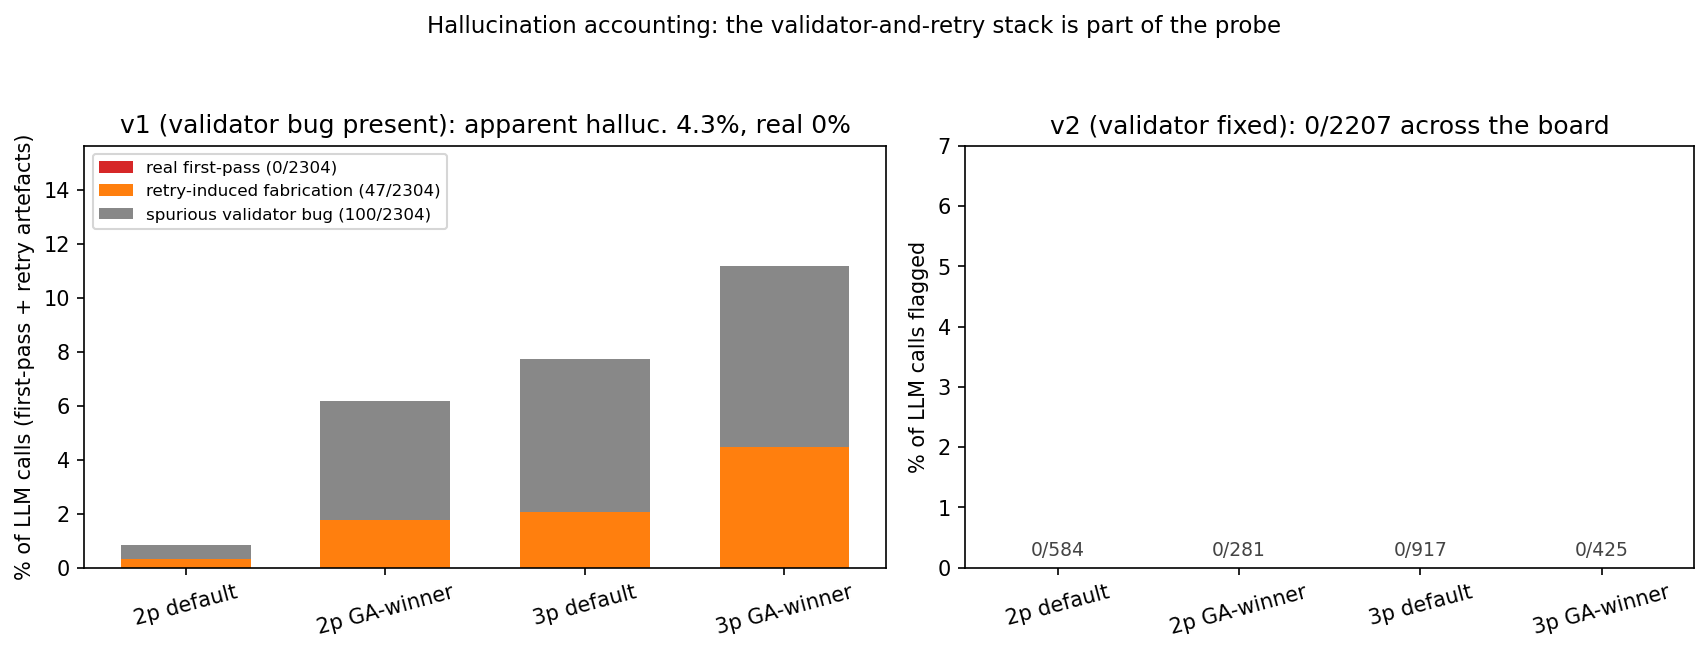
\includegraphics[width=0.78\linewidth]{llm/fig_v1_vs_v2_hallucination.png}
\caption{\textbf{Structured echo validation eliminates state
hallucinations.} Per-call validation outcomes for the v1 free-form
prompt and the v2 structured \texttt{STATE/ECHO/REASON/ANSWER}
prompt with deterministic per-field equality checking on the echoed
state. v1 produces a non-trivial fraction of calls in which the
model's reasoning references state that does not appear in the
prompt. v2 drives that bar to zero across all $2{,}288$ calls, at the
cost of a small additional retry budget. This is the precondition
for treating the LLM as a trustworthy independent agent class in
everything that follows: a benchmark whose probe fabricates inputs
is not measuring what it claims to measure.}
\label{fig:hallucination}
\end{figure}

\begin{figure}[h!]
\centering

\includegraphics[width=0.78\linewidth]{llm/fig_cross_class_agreement.png}
\caption{\textbf{The trustworthy LLM probe agrees with the rule-based
pool on the directional ranking of boards.} Per metric (rounds,
fairness, draws, transfer), bars compare the value on the default
board against the GA-2p winning board, scored under the 30-strategy
rule-based pool and under the all-LLM probe. On every metric with a
clean ordering, both evaluators move in the same direction and by
similar relative magnitudes: the optimisation effect identified by
the rule-based pool reproduces under an independent agent class.
Absolute composite scores are not directly comparable across
evaluators because the LLM is a single personality and the rule-based
pool is 30 distinct ones, which is the limitation we revisit in
Section~\ref{sec:llm_ga}.}
\label{fig:agreement}
\end{figure}

The v1 prompt exposed a second-order finding worth reporting in its
own right. v1's validator had a subtle integer/float type mismatch in
the cash field, and retries against a wrong validator induced
\emph{more} plausible-looking confabulation rather than less, because
the model was being told a correct value was wrong and produced a
different ``corrected'' answer to satisfy the validator. We document
this rather than tuning the validator until it disappears: a protocol
whose failure modes are reported alongside its results is auditable;
one whose are not is a benchmark trick.

\begin{figure}[h!]
\centering
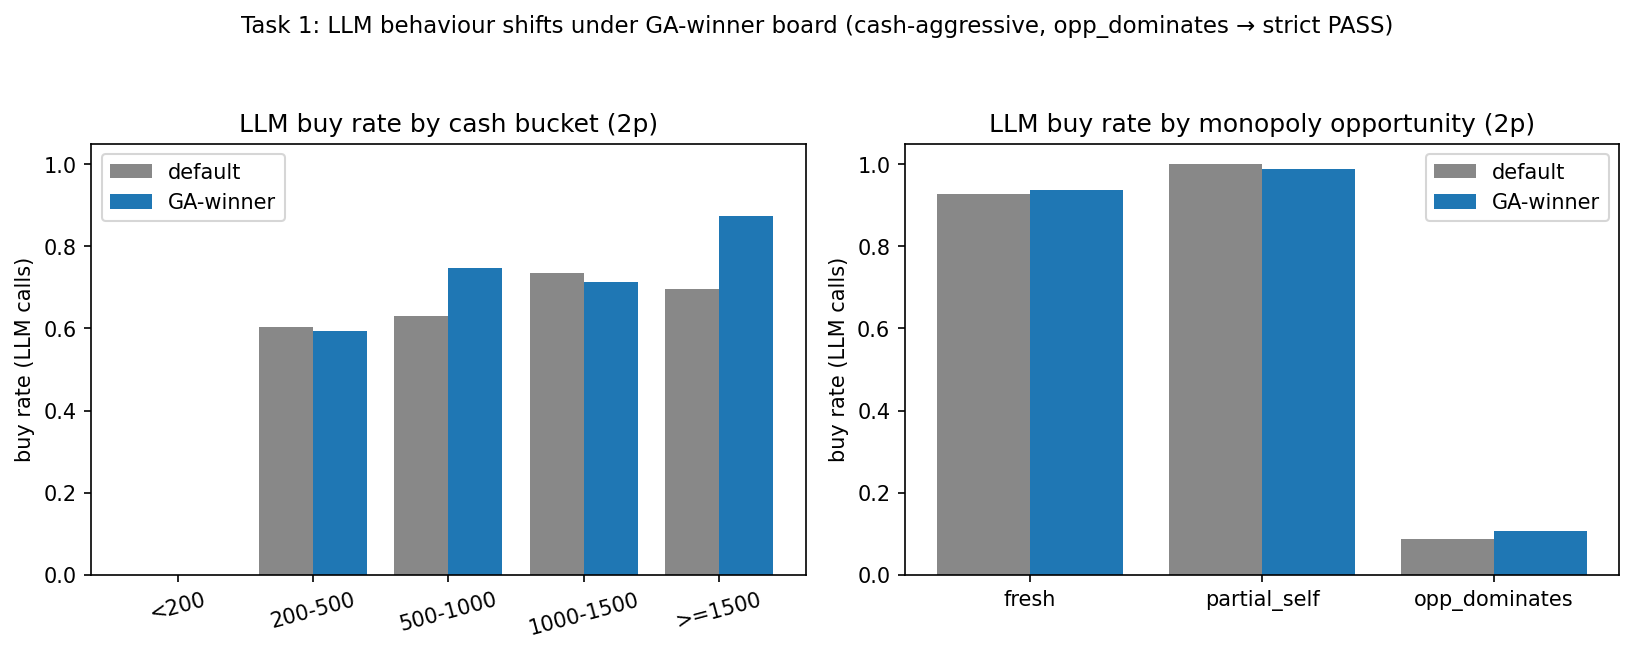
\includegraphics[width=0.78\linewidth]{llm/fig_llm_buy_rate_slices.png}
\caption{\textbf{LLM buy-rate slices, default board vs.\ GA-2p
winner.} \textbf{(a)~By cash bucket.} Buy rate conditioned on the
LLM's available cash at decision time. The rate rises monotonically
with cash, the rational ordering for any non-degenerate strategy;
the empty $<200$ bucket reflects the affordability pre-filter that
short-circuits the LLM call when the player cannot buy anyway. On
the GA-winner board the LLM commits its cash hoard more aggressively
in the $\geq 1500$ bucket ($\sim 0.87$ vs.\ $\sim 0.70$ on the
default), so the optimised board successfully pulls behaviour out of
the cash-hoarding regime. \textbf{(b)~By monopoly-completion
situation.} \textsl{fresh}: no player owns any property in the
landed colour group, so a purchase starts a new collection.
\textsl{partial\_self}: the LLM already owns one or more properties
in the group and the opponent does not dominate it.
\textsl{opp\_dominates}: the opponent owns at least half the group
and at least as many properties as the LLM, so buying mostly funds
their next rent payment. Buy rates respond rationally across all
three: $\sim 1.00$ on \textsl{partial\_self} (saturated buy),
$\sim 0.94$ on \textsl{fresh}, and $\sim 0.10$ on
\textsl{opp\_dominates} (strict PASS). The probe is not behaving as
a uniform random oracle, and the directional responses are
essentially identical on both boards.}
\label{fig:slices}
\end{figure}

\subsection{LLM-driven GA and the fairness gap}\label{sec:llm_ga}

We re-ran the GA with the LLM as evaluator (population 8, 5
generations, 5 seeds per candidate, 2-player only). The LLM-GA
converges (Figure~\ref{fig:llm_ga_conv}) and produces a winning board
that beats the default under all-LLM evaluation. Cross-evaluating
that board under the rule-based pool produces the diagnostic finding
of the project (Figure~\ref{fig:gap}): the LLM-GA winner is better
than the default under either evaluator, but loses to the rule-based
GA winner under the diverse pool. The fairness gap is $0.20$ vs.\
$0.379$ at 2p and $0.05$ vs.\ $0.404$ at 3p, and \emph{widens} with
more identical seats.

\begin{figure}[h!]
\centering
\begin{subfigure}[t]{0.48\linewidth}\centering
  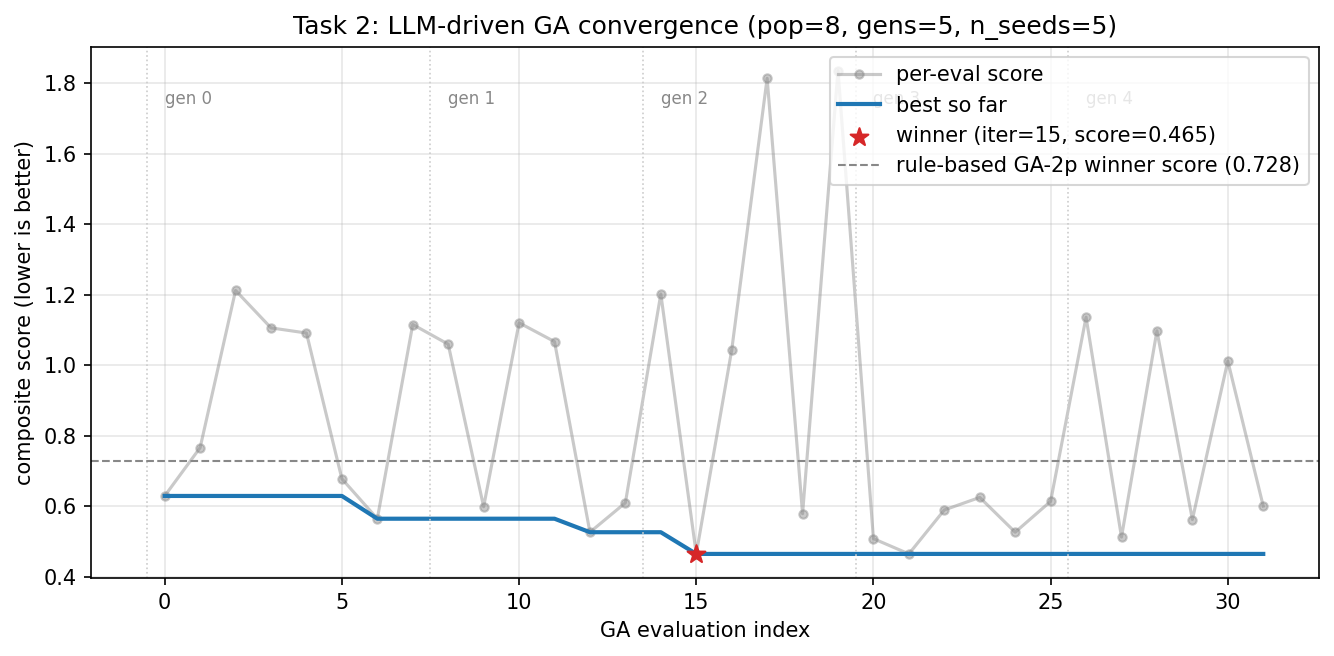
\includegraphics[width=\linewidth]{llm/fig_llm_ga_convergence.png}
  \caption{LLM-GA best-so-far}
\end{subfigure}\hfill
\begin{subfigure}[t]{0.48\linewidth}\centering
  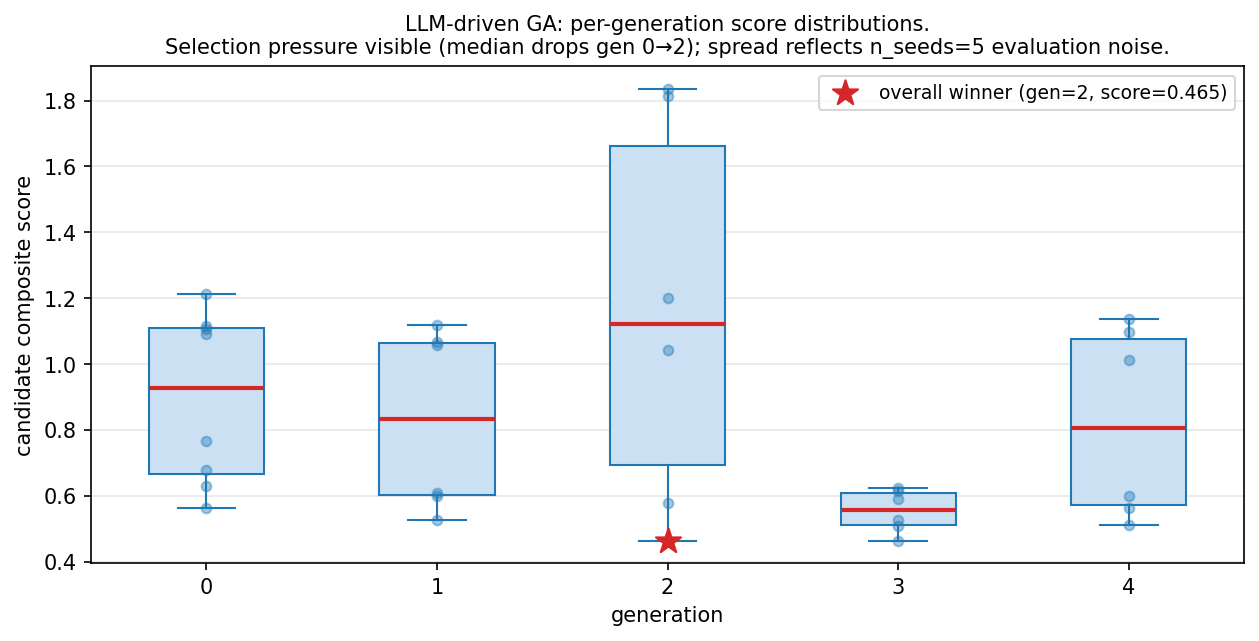
\includegraphics[width=\linewidth]{llm/fig_llm_ga_score_distribution.png}
  \caption{Score distribution}
\end{subfigure}
\caption{\textbf{An LLM-only evaluator can drive the same GA loop to
a non-trivial design.} \textbf{(a)}~Best-so-far composite score over
LLM-GA evaluation count (population~$8 \times 5$ generations $\times
5$ seeds, 2-player only). \textbf{(b)}~Score distribution across all
evaluations, with the default-board reference and the LLM-GA winner
marked. The loop converges within budget and produces a board that
beats the default under all-LLM evaluation; the narrowing
generation-$3$-to-$5$ gap signals the search approaching a local
plateau. Total wall time $4$h~$58$min on a single $12$~GB GPU.
Whether the converged board is a real design optimum or only an
LLM-evaluator optimum is the question Figure~\ref{fig:gap}
resolves.}
\label{fig:llm_ga_conv}
\end{figure}

\begin{figure}[h!]
\centering
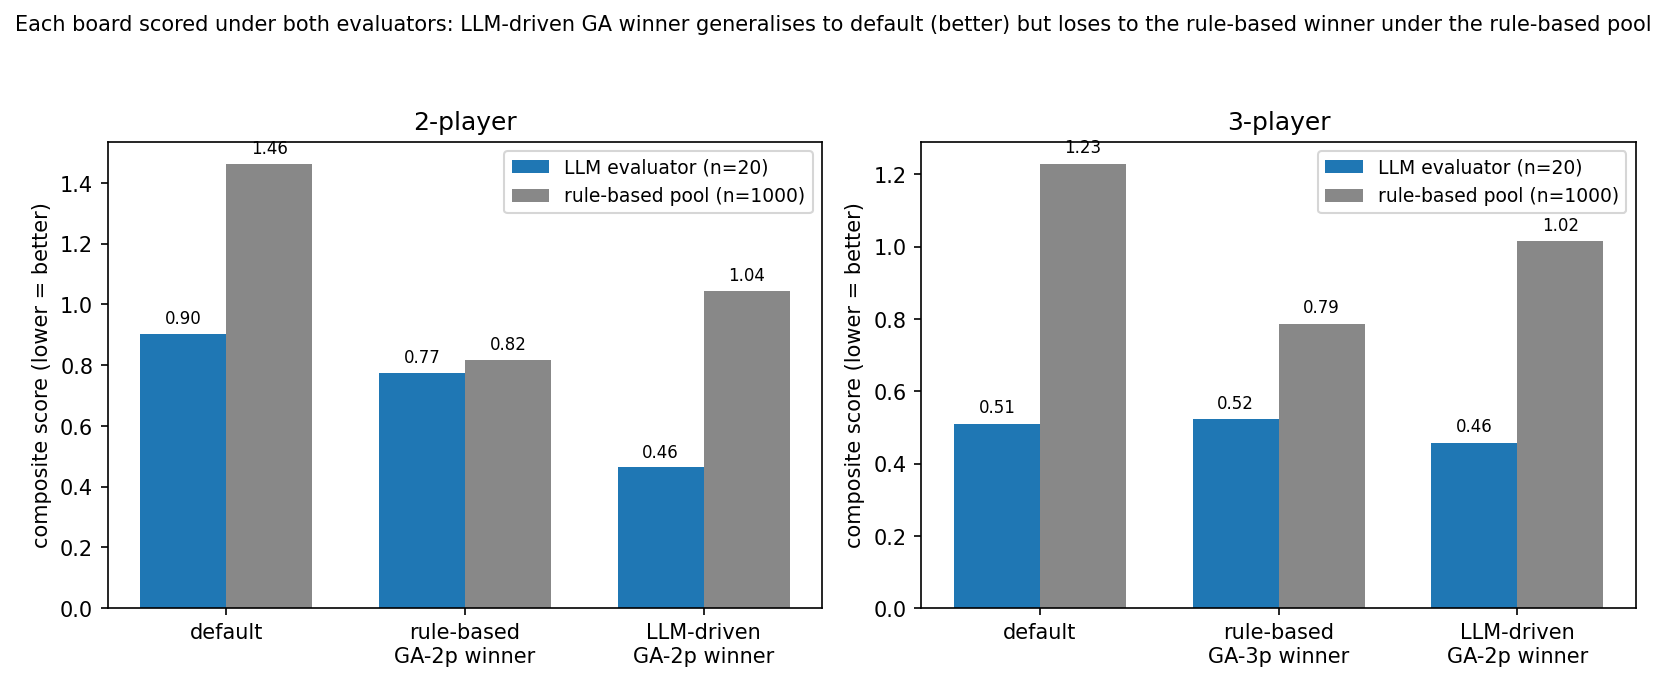
\includegraphics[width=0.92\linewidth]{llm/fig_cross_evaluator_gap.png}
\caption{\textbf{Headline diagnostic: a single-personality evaluator
misses the worst-case fairness term that a strategy pool catches.}
A $2{\times}2$ grid scores three boards (default, rule-based GA
winner, LLM-GA winner) on two metrics (rounds, fairness) under both
evaluators (the 30-strategy rule-based pool, and an all-LLM
evaluator), at 2 and 3 players. The LLM-GA winner improves on the
default under either evaluator on both metrics, so the LLM-driven
optimiser is not broken; but it loses to the rule-based GA winner on
fairness under the diverse pool, with a gap of $0.20$ vs.\ $0.379$
at 2p and $0.05$ vs.\ $0.404$ at 3p. The gap \emph{widens} with
player count: more identical seats produce more correlated mistakes
for a single-personality evaluator, and the strategy pool's
diversity is what protects against them. This is the central
empirical claim of the paper: evaluator diversity is not optional
for fairness-sensitive design.}
\label{fig:gap}
\end{figure}

\begin{figure}[h!]
\centering
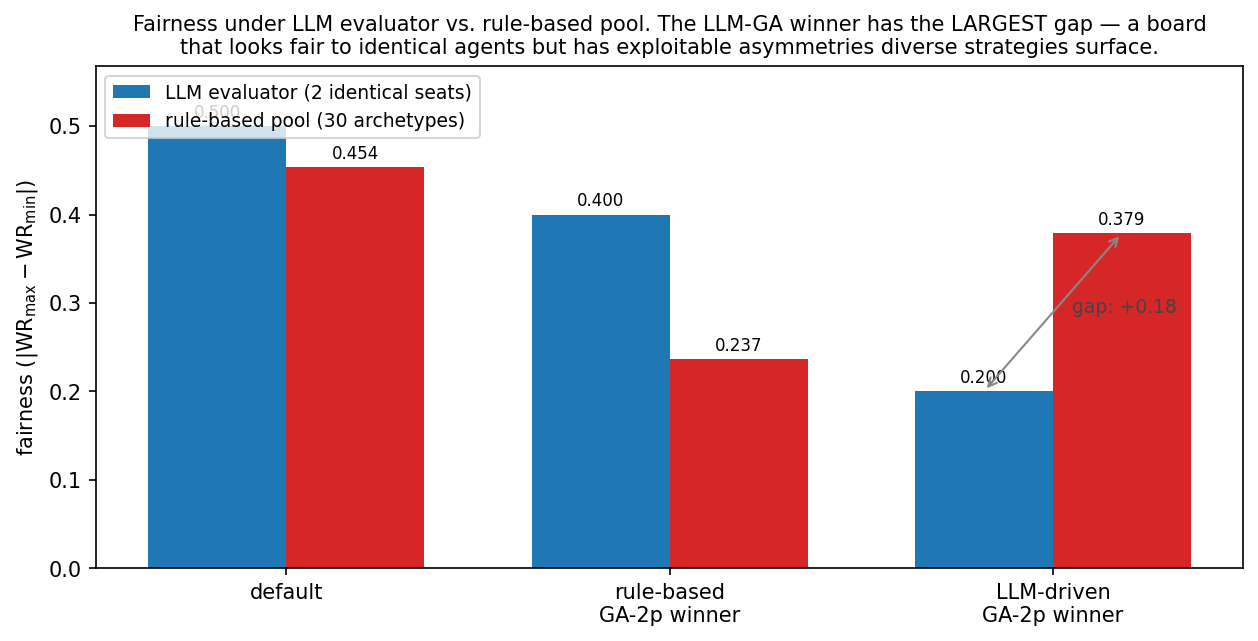
\includegraphics[width=0.78\linewidth]{llm/fig_fairness_asymmetry.png}
\caption{\textbf{The seat-level mechanism behind the cross-evaluator
gap.} Per-seat win rates on the LLM-GA winning board under all-LLM
evaluation (P0, P1 at 2p; P0, P1, P2 at 3p). With identical agents
in every seat, win rates should be uniform; instead a single seat
consistently wins more than the others. The 30-strategy rule-based
pool averages this kind of single-agent bias out across diverse
playstyles, but a single LLM evaluator cannot, which is exactly the
mechanism that produces the cross-evaluator fairness gap in
Figure~\ref{fig:gap}.}
\label{fig:asymmetry}
\end{figure}

The interpretation is straightforward and is the headline diagnostic
of the project: the LLM is good enough to drive an optimiser to a
non-trivial design, but using a \emph{single} agent personality as the
evaluator collapses the worst-case fairness term. Evaluator diversity
is therefore not optional for fairness-sensitive design. A single LLM
or RL agent as evaluator is a benchmark; a strategy pool is a
beta-testing surrogate.

\subsection{Reproducibility check}\label{sec:repro}

Re-running any $(\theta, \text{matchups}, \text{seeds})$ triple yields
byte-identical metrics. We verified this by re-running two randomly
chosen JSONL lines from each major run and diffing the outputs. Every
number in this report can be regenerated from a seed plus a JSONL
line; the seed schedule is recorded in each run's
\texttt{meta.json}.

\subsection{Limitations}\label{sec:lim}

\begin{itemize}[leftmargin=1.2em,itemsep=1pt]
\item \textbf{Strategy-pool coverage.} The 17-dim parametric space is
broad but not exhaustive, and human players behave outside it. The 20
sampled strategies broaden the pool beyond the 10 archetypes and the
sampling procedure is documented and reproducible, but a real
deployment would want to learn the strategy distribution from logs.
\item \textbf{Phase B not run.} Human playtesting is pre-declared but
not executed in this report. The falsifiability claim is accordingly
limited: two agent classes agree directionally; whether either class
predicts human play remains untested.
\item \textbf{LLM scale.} Qwen2.5-1.5B is the only LLM in the study.
Larger models or different prompt styles may change the agreement
profile. Greedy decoding does, however, make the probe deterministic.
\item \textbf{Single-board scope.} All optimisation runs on the
standard 40-cell US Monopoly layout (with structural shrinkage via
keep-mask). Other game families would require a new design-space
encoder, but the rest of the pipeline (objective, pool, GA,
validator) carries over unchanged.
\end{itemize}

\subsection{Lessons for multi-agent system design}\label{sec:lessons}

\begin{enumerate}[leftmargin=1.4em,itemsep=1pt]
\item \textbf{Strategy-pool diversity beats single oracle.} A
$30$-strategy parametric pool is a more honest evaluator than the
strongest single agent we can train in the same time budget; the
cross-evaluator gap (Section~\ref{sec:llm_ga}) is the empirical
evidence.
\item \textbf{Robust aggregation belongs in the objective.} A
worst-pair fairness term ($F_{\max}$) prevents the optimiser from
improving the average at the expense of the tail; CVaR or a hard
$\min$ generalise the same idea further.
\item \textbf{Per-objective ablations expose redundancy.} If two terms
drive the same optimum, drop one; if they drive different optima
(this work), keep both and report the trade-off explicitly.
\item \textbf{Evaluation context is itself a design variable.} The 2p
and 3p winners do not coincide; an optimisation result claimed under
one regime should be re-evaluated under counterfactual conditions
before it ships.
\item \textbf{Variance reduction beats more samples.} Shared random
numbers across candidates made GA convergence visible at $100$ games
per candidate; uncorrelated evaluations would have required
$\sim 1000$ games for the same signal.
\item \textbf{The validator-and-retry stack is part of the probe.}
v1's retry-induced fabrication is documented as a finding rather than
patched away; a benchmark whose failure modes are not reported is a
benchmark trick.
\end{enumerate}

% =====================================================================
\section{Team responsibilities}\label{sec:team}
% =====================================================================

\paragraph{Selim Emir Can.} % TODO: confirm or edit
Closed-loop optimisation pipeline (\texttt{ParametricPlayer}, strategy
pool, design space, simulator wrapper, objectives, GA); LLM probe
layer (\texttt{LLMPlayer}, structured \texttt{STATE/ECHO/REASON/
ANSWER} prompt, deterministic per-field validator, retry loop,
per-decision logging); Task~1 (LLM-only Phase~C eval) and Task~2
(LLM-driven GA); cross-evaluation harness; figure generation; report
writing.

\paragraph{Alaz Cig.} % TODO: please fill in / replace
[FILL IN: 1--2 sentences on Alaz's contributions. The git history
on the \texttt{round1-phase1} and \texttt{main} branches contains
parallel work I did not have visibility into; please replace this
placeholder with the canonical breakdown before submission.]

% =====================================================================
% \section*{References}
% =====================================================================
% Lightweight \thebibliography rather than BibTeX so the file
% compiles standalone. Replace or extend as the final list firms up.
\begin{thebibliography}{9}

\bibitem{qwen25}
Qwen Team.
\textit{Qwen2.5 Technical Report}.
2024.

\bibitem{pettingzoo}
J.~K. Terry et al.
\textit{PettingZoo: A Standard API for Multi-Agent Reinforcement
Learning}. NeurIPS, 2021.

\bibitem{ga-goldberg}
D.~E. Goldberg.
\textit{Genetic Algorithms in Search, Optimization, and Machine
Learning}. Addison-Wesley, 1989.

\bibitem{crn}
A.~M. Law and W.~D. Kelton.
\textit{Simulation Modeling and Analysis}, chapter on Common Random
Numbers. McGraw-Hill, 5th ed., 2014.

\bibitem{wilson}
E.~B. Wilson.
\textit{Probable Inference, the Law of Succession, and Statistical
Inference}. JASA, 1927.

\end{thebibliography}

\end{document}
